% Options for packages loaded elsewhere
\PassOptionsToPackage{unicode}{hyperref}
\PassOptionsToPackage{hyphens}{url}
\PassOptionsToPackage{dvipsnames,svgnames,x11names}{xcolor}
%
\documentclass[
  letterpaper,
  DIV=11,
  numbers=noendperiod]{scrreprt}

\usepackage{amsmath,amssymb}
\usepackage{iftex}
\ifPDFTeX
  \usepackage[T1]{fontenc}
  \usepackage[utf8]{inputenc}
  \usepackage{textcomp} % provide euro and other symbols
\else % if luatex or xetex
  \usepackage{unicode-math}
  \defaultfontfeatures{Scale=MatchLowercase}
  \defaultfontfeatures[\rmfamily]{Ligatures=TeX,Scale=1}
\fi
\usepackage{lmodern}
\ifPDFTeX\else  
    % xetex/luatex font selection
\fi
% Use upquote if available, for straight quotes in verbatim environments
\IfFileExists{upquote.sty}{\usepackage{upquote}}{}
\IfFileExists{microtype.sty}{% use microtype if available
  \usepackage[]{microtype}
  \UseMicrotypeSet[protrusion]{basicmath} % disable protrusion for tt fonts
}{}
\makeatletter
\@ifundefined{KOMAClassName}{% if non-KOMA class
  \IfFileExists{parskip.sty}{%
    \usepackage{parskip}
  }{% else
    \setlength{\parindent}{0pt}
    \setlength{\parskip}{6pt plus 2pt minus 1pt}}
}{% if KOMA class
  \KOMAoptions{parskip=half}}
\makeatother
\usepackage{xcolor}
\setlength{\emergencystretch}{3em} % prevent overfull lines
\setcounter{secnumdepth}{5}
% Make \paragraph and \subparagraph free-standing
\ifx\paragraph\undefined\else
  \let\oldparagraph\paragraph
  \renewcommand{\paragraph}[1]{\oldparagraph{#1}\mbox{}}
\fi
\ifx\subparagraph\undefined\else
  \let\oldsubparagraph\subparagraph
  \renewcommand{\subparagraph}[1]{\oldsubparagraph{#1}\mbox{}}
\fi

\usepackage{color}
\usepackage{fancyvrb}
\newcommand{\VerbBar}{|}
\newcommand{\VERB}{\Verb[commandchars=\\\{\}]}
\DefineVerbatimEnvironment{Highlighting}{Verbatim}{commandchars=\\\{\}}
% Add ',fontsize=\small' for more characters per line
\usepackage{framed}
\definecolor{shadecolor}{RGB}{241,243,245}
\newenvironment{Shaded}{\begin{snugshade}}{\end{snugshade}}
\newcommand{\AlertTok}[1]{\textcolor[rgb]{0.68,0.00,0.00}{#1}}
\newcommand{\AnnotationTok}[1]{\textcolor[rgb]{0.37,0.37,0.37}{#1}}
\newcommand{\AttributeTok}[1]{\textcolor[rgb]{0.40,0.45,0.13}{#1}}
\newcommand{\BaseNTok}[1]{\textcolor[rgb]{0.68,0.00,0.00}{#1}}
\newcommand{\BuiltInTok}[1]{\textcolor[rgb]{0.00,0.23,0.31}{#1}}
\newcommand{\CharTok}[1]{\textcolor[rgb]{0.13,0.47,0.30}{#1}}
\newcommand{\CommentTok}[1]{\textcolor[rgb]{0.37,0.37,0.37}{#1}}
\newcommand{\CommentVarTok}[1]{\textcolor[rgb]{0.37,0.37,0.37}{\textit{#1}}}
\newcommand{\ConstantTok}[1]{\textcolor[rgb]{0.56,0.35,0.01}{#1}}
\newcommand{\ControlFlowTok}[1]{\textcolor[rgb]{0.00,0.23,0.31}{#1}}
\newcommand{\DataTypeTok}[1]{\textcolor[rgb]{0.68,0.00,0.00}{#1}}
\newcommand{\DecValTok}[1]{\textcolor[rgb]{0.68,0.00,0.00}{#1}}
\newcommand{\DocumentationTok}[1]{\textcolor[rgb]{0.37,0.37,0.37}{\textit{#1}}}
\newcommand{\ErrorTok}[1]{\textcolor[rgb]{0.68,0.00,0.00}{#1}}
\newcommand{\ExtensionTok}[1]{\textcolor[rgb]{0.00,0.23,0.31}{#1}}
\newcommand{\FloatTok}[1]{\textcolor[rgb]{0.68,0.00,0.00}{#1}}
\newcommand{\FunctionTok}[1]{\textcolor[rgb]{0.28,0.35,0.67}{#1}}
\newcommand{\ImportTok}[1]{\textcolor[rgb]{0.00,0.46,0.62}{#1}}
\newcommand{\InformationTok}[1]{\textcolor[rgb]{0.37,0.37,0.37}{#1}}
\newcommand{\KeywordTok}[1]{\textcolor[rgb]{0.00,0.23,0.31}{#1}}
\newcommand{\NormalTok}[1]{\textcolor[rgb]{0.00,0.23,0.31}{#1}}
\newcommand{\OperatorTok}[1]{\textcolor[rgb]{0.37,0.37,0.37}{#1}}
\newcommand{\OtherTok}[1]{\textcolor[rgb]{0.00,0.23,0.31}{#1}}
\newcommand{\PreprocessorTok}[1]{\textcolor[rgb]{0.68,0.00,0.00}{#1}}
\newcommand{\RegionMarkerTok}[1]{\textcolor[rgb]{0.00,0.23,0.31}{#1}}
\newcommand{\SpecialCharTok}[1]{\textcolor[rgb]{0.37,0.37,0.37}{#1}}
\newcommand{\SpecialStringTok}[1]{\textcolor[rgb]{0.13,0.47,0.30}{#1}}
\newcommand{\StringTok}[1]{\textcolor[rgb]{0.13,0.47,0.30}{#1}}
\newcommand{\VariableTok}[1]{\textcolor[rgb]{0.07,0.07,0.07}{#1}}
\newcommand{\VerbatimStringTok}[1]{\textcolor[rgb]{0.13,0.47,0.30}{#1}}
\newcommand{\WarningTok}[1]{\textcolor[rgb]{0.37,0.37,0.37}{\textit{#1}}}

\providecommand{\tightlist}{%
  \setlength{\itemsep}{0pt}\setlength{\parskip}{0pt}}\usepackage{longtable,booktabs,array}
\usepackage{calc} % for calculating minipage widths
% Correct order of tables after \paragraph or \subparagraph
\usepackage{etoolbox}
\makeatletter
\patchcmd\longtable{\par}{\if@noskipsec\mbox{}\fi\par}{}{}
\makeatother
% Allow footnotes in longtable head/foot
\IfFileExists{footnotehyper.sty}{\usepackage{footnotehyper}}{\usepackage{footnote}}
\makesavenoteenv{longtable}
\usepackage{graphicx}
\makeatletter
\def\maxwidth{\ifdim\Gin@nat@width>\linewidth\linewidth\else\Gin@nat@width\fi}
\def\maxheight{\ifdim\Gin@nat@height>\textheight\textheight\else\Gin@nat@height\fi}
\makeatother
% Scale images if necessary, so that they will not overflow the page
% margins by default, and it is still possible to overwrite the defaults
% using explicit options in \includegraphics[width, height, ...]{}
\setkeys{Gin}{width=\maxwidth,height=\maxheight,keepaspectratio}
% Set default figure placement to htbp
\makeatletter
\def\fps@figure{htbp}
\makeatother
\newlength{\cslhangindent}
\setlength{\cslhangindent}{1.5em}
\newlength{\csllabelwidth}
\setlength{\csllabelwidth}{3em}
\newlength{\cslentryspacingunit} % times entry-spacing
\setlength{\cslentryspacingunit}{\parskip}
\newenvironment{CSLReferences}[2] % #1 hanging-ident, #2 entry spacing
 {% don't indent paragraphs
  \setlength{\parindent}{0pt}
  % turn on hanging indent if param 1 is 1
  \ifodd #1
  \let\oldpar\par
  \def\par{\hangindent=\cslhangindent\oldpar}
  \fi
  % set entry spacing
  \setlength{\parskip}{#2\cslentryspacingunit}
 }%
 {}
\usepackage{calc}
\newcommand{\CSLBlock}[1]{#1\hfill\break}
\newcommand{\CSLLeftMargin}[1]{\parbox[t]{\csllabelwidth}{#1}}
\newcommand{\CSLRightInline}[1]{\parbox[t]{\linewidth - \csllabelwidth}{#1}\break}
\newcommand{\CSLIndent}[1]{\hspace{\cslhangindent}#1}

\KOMAoption{captions}{tableheading}
\makeatletter
\makeatother
\makeatletter
\@ifpackageloaded{bookmark}{}{\usepackage{bookmark}}
\makeatother
\makeatletter
\@ifpackageloaded{caption}{}{\usepackage{caption}}
\AtBeginDocument{%
\ifdefined\contentsname
  \renewcommand*\contentsname{Table of contents}
\else
  \newcommand\contentsname{Table of contents}
\fi
\ifdefined\listfigurename
  \renewcommand*\listfigurename{List of Figures}
\else
  \newcommand\listfigurename{List of Figures}
\fi
\ifdefined\listtablename
  \renewcommand*\listtablename{List of Tables}
\else
  \newcommand\listtablename{List of Tables}
\fi
\ifdefined\figurename
  \renewcommand*\figurename{Figure}
\else
  \newcommand\figurename{Figure}
\fi
\ifdefined\tablename
  \renewcommand*\tablename{Table}
\else
  \newcommand\tablename{Table}
\fi
}
\@ifpackageloaded{float}{}{\usepackage{float}}
\floatstyle{ruled}
\@ifundefined{c@chapter}{\newfloat{codelisting}{h}{lop}}{\newfloat{codelisting}{h}{lop}[chapter]}
\floatname{codelisting}{Listing}
\newcommand*\listoflistings{\listof{codelisting}{List of Listings}}
\makeatother
\makeatletter
\@ifpackageloaded{caption}{}{\usepackage{caption}}
\@ifpackageloaded{subcaption}{}{\usepackage{subcaption}}
\makeatother
\makeatletter
\@ifpackageloaded{tcolorbox}{}{\usepackage[skins,breakable]{tcolorbox}}
\makeatother
\makeatletter
\@ifundefined{shadecolor}{\definecolor{shadecolor}{rgb}{.97, .97, .97}}
\makeatother
\makeatletter
\makeatother
\makeatletter
\makeatother
\ifLuaTeX
  \usepackage{selnolig}  % disable illegal ligatures
\fi
\IfFileExists{bookmark.sty}{\usepackage{bookmark}}{\usepackage{hyperref}}
\IfFileExists{xurl.sty}{\usepackage{xurl}}{} % add URL line breaks if available
\urlstyle{same} % disable monospaced font for URLs
\hypersetup{
  pdftitle={Correcting Effect Sizes for Statistical Artifacts},
  pdfauthor={Matthew B. Jané},
  colorlinks=true,
  linkcolor={blue},
  filecolor={Maroon},
  citecolor={Blue},
  urlcolor={Blue},
  pdfcreator={LaTeX via pandoc}}

\title{Correcting Effect Sizes for Statistical Artifacts}
\usepackage{etoolbox}
\makeatletter
\providecommand{\subtitle}[1]{% add subtitle to \maketitle
  \apptocmd{\@title}{\par {\large #1 \par}}{}{}
}
\makeatother
\subtitle{Application in Meta-Analysis and Implementation in R and
Python}
\author{Matthew B. Jané}
\date{2023-06-13}

\begin{document}
\maketitle
\ifdefined\Shaded\renewenvironment{Shaded}{\begin{tcolorbox}[interior hidden, borderline west={3pt}{0pt}{shadecolor}, breakable, enhanced, sharp corners, frame hidden, boxrule=0pt]}{\end{tcolorbox}}\fi

\renewcommand*\contentsname{Table of contents}
{
\hypersetup{linkcolor=}
\setcounter{tocdepth}{2}
\tableofcontents
}
\bookmarksetup{startatroot}

\hypertarget{proposal-and-outline}{%
\chapter{Proposal and Outline}\label{proposal-and-outline}}

Results across scientific studies vary drastically even when studying
the same underlying phenomena. Sometimes these can be accounted for by
some study-level characteristic (i.e., methodology, population, etc.) or
it can be accounted for by variations in statistical artifacts such as
measurement error or selection effects. Not only does the heterogeneity
increase in the presence of statistical artifacts, but artifacts also
induce systematic biases that can cause inaccurate results. Artifacts
restrict our ability to draw meaningful inferences from scientific
results, therefore it is important to apply corrections in order to
obtain unbiased estimates.

\textbf{Overview.} The goal of the general exam is to turn it into an
online open source e-textbook similar to
\href{https://bookdown.org/MathiasHarrer/Doing_Meta_Analysis_in_R/}{this
one on meta-analysis in R} by Mathias Harrer and colleagues. The e-text
will be split into two parts: artifact corrections and their application
to meta-analysis. Each type of artifact will have a section of its own
that details the history, methodology, and its implementation in R and
Python. Another section will be dedicated to applying artifact
corrections to meta-analysis, which is the type of research where the
corrections are most used. The meta-analysis section will also contain
the four parts (history, methodology, assumptions, and implementation in
R). See \href{https://MatthewBJane.github.io/artifact-corrections}{this
webpage} where I cataloged equations and code that will go into this
general exam. I also have started writing the
\protect\hyperlink{unreliability}{unreliability section} so you can
start get an idea of how this will look.

\textbf{History.} The history part will provide an overview of the
literature for that artifact correction. It will note where the
correction first was introduced, the adjustments people have made since
then, as well as studies where the correction has been applied (most
likely in a meta-analysis). Also if applicable, provide examples of
where these meta-analyses have utilized such corrections (e.g., Roth et
al., 2015) Methodology. The methodological part will review the
correction equations (for point estimates and standard errors) and how
they were derived for each artifact correction. Artifact corrections
will be applied to both correlation coefficients and standardized mean
differences (repeated measures and independent samples). The
methodological part for the meta-analysis section will discuss how
heterogeneity, credibility/confidence intervals, and averages are
calculated in the context of artifact corrections. It will also touch on
competing approaches (Raju et al., 1983) to the traditional artifact
correction approaches (Hunter \& Schmidt, 2004).

\textbf{Assumptions.} Each artifact correction contains assumptions that
must be met in order to obtain unbiased estimate of the true population
effect size. This part will discuss each of these assumptions, when each
matter, and what simulation studies have found in regard to violation of
assumptions. Assumptions at the meta-analytic level of analysis (e.g.,
independence between artifacts and moderators) will also be discussed.

\textbf{Implementation in R and Python.} Artifact corrections are only
useful if you can apply them. Since many of the corrections are quite
complex, it is important that these can be implemented easily in an
open-source software such as R and Python. Each correction will be
supplemented with code using R and Python with some additional packages
like psychmeta (Dahlke and Wiernik 2019). For statistical analyses and
especially for meta-analysis, R has tremendous support in terms of
useful packages and a large community that makes it a highly flexible
and powerful language. Python is a general-purpose programming language
that is a more popular than R. For an example of how this will be done
see this section on
\protect\hyperlink{estimating-reliability-code}{estimating reliability
in R and Python.}

\bookmarksetup{startatroot}

\hypertarget{dedication}{%
\chapter{Dedication}\label{dedication}}

In Loving Memory of Haley Jané

My companion whose unwavering presence and unconditional love provided
me with stability and solace in life's ever-changing journey

\begin{figure}

{\centering 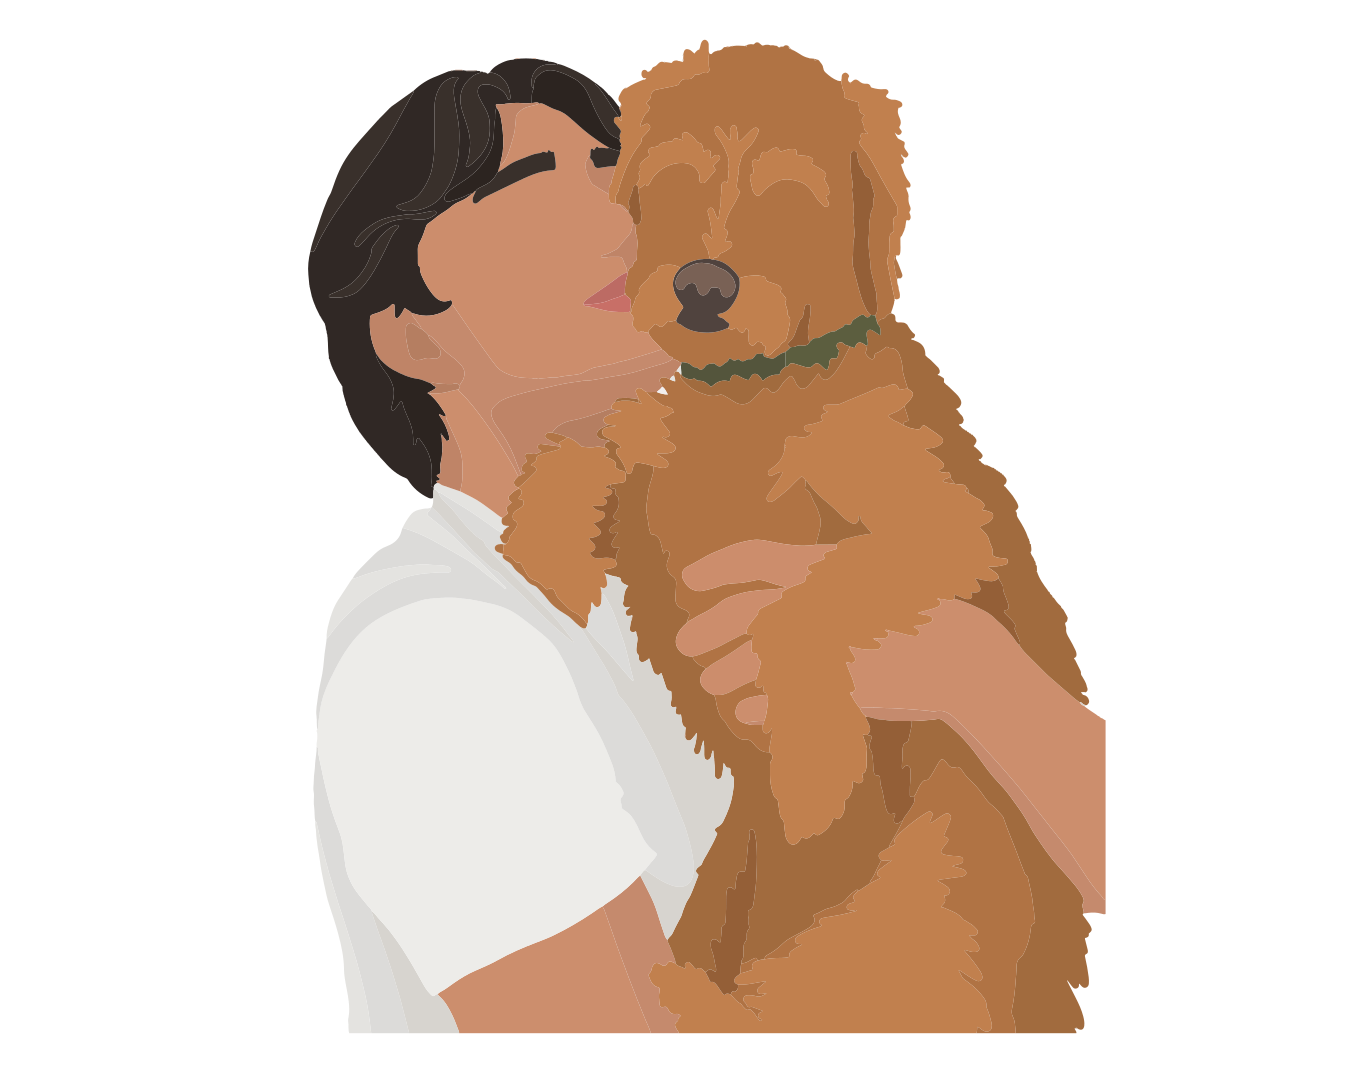
\includegraphics[width=4.16667in,height=\textheight]{figure/dedication_2.png}

}

\end{figure}

\bookmarksetup{startatroot}

\hypertarget{introduction}{%
\chapter{Introduction}\label{introduction}}

\hypertarget{effect-sizes}{%
\section{Effect Sizes}\label{effect-sizes}}

\hypertarget{correlations}{%
\subsection{Correlations}\label{correlations}}

A correlation describes the relationship between two continuous
variables. The correlation coefficient was first introduced 1904 by
Charles Spearman

\hypertarget{technical-overview}{%
\subsubsection*{Technical Overview}\label{technical-overview}}
\addcontentsline{toc}{subsubsection}{Technical Overview}

If we draw a sample of \(n\) observations from a population, we can
estimate the population correlation between variables \(x\) and \(y\)
using a reasonably unbiased estimator, \(r\),

\[
r = \frac{
\sum_{i=1}^{n}(x_i - \bar{x})(y_i - \bar{y})
}{
\sqrt{\sum_{i=1}^{n}(x_i - \bar{x})^2}
\sqrt{\sum_{i=1}^{n}(x_i - \bar{x})^2}
}
\]This formulation is commonly referred to as the Pearson correlation
coefficient (\textbf{pe?}) . To see under the hood of this seemingly
complex mathematical formulation. Since the correlation is simply the
the standardized covariance between two variables, x and y, we can first
define the covariance as the product of the squared errors between
(\(x_i - \bar{x}\)) and y (\(y_i - \bar{y}\)),

\[
\sigma_{xy} =\frac{1}{n-1}\sum_{i=1}^{n}(x_i - \bar{x})(y_i - \bar{y})
\]

Then we can find the variance for x and y by taking the average squared
error from the mean for x and y,

\[
\sigma_x = \sqrt{\frac{1}{n-1}\sum_{i=1}^n (x_i - \bar{x})}
\]

\[
\sigma_y = \sqrt{\frac{1}{n-1}\sum_{i=1}^n (y_i - \bar{y})}
\]

Now with each of these components, we can standardized the covariance by
dividing by the standard deviations of x and y (i.e., square root of the
variance). It can be now seen that the \(\frac{1}{n-1}\) term cancels
out in the numerator and denominator and thus will give us the original
formula for the sample correlation coefficient.

\begin{equation}\protect\hypertarget{eq-1}{}{
r = \frac{\sigma_{xy}}{\sigma_x\sigma_y} = \frac{\sum_{i=1}^{n}(x_i - \bar{x})(y_i - \bar{y})}{\sqrt{\sum_{i=1}^{n}(x_i - \bar{x})^2}\sqrt{\sum_{i=1}^{n}(x_i - \bar{x})^2}}
}\label{eq-1}\end{equation}

Since \(r\) is the observed sample correlation, it is important to note
that, in the absence of artifacts, \(r\) provides an unbiased estimate
of the true population correlation \(\rho\) (\(r =\hat{\rho}\)).
Therefore, in conditions uncontaminated by artifacts, differences
between the observed sample correlation and the true population
correlation are attributable to sampling error (\(\varepsilon\)) such
that,

\begin{equation}\protect\hypertarget{eq-2}{}{
\rho = \hat{\rho} + \varepsilon = r + \varepsilon
}\label{eq-2}\end{equation} Where \(se_r\) is the standard error of the
observed correlation. The standard error can be calculated from the
sample size (\(n\)) and the observed correlation,
\begin{equation}\protect\hypertarget{eq-3}{}{
se_r =\sqrt{\frac{1 - r^2}{n-2}} 
}\label{eq-3}\end{equation}

\hypertarget{standardized-mean-differences}{%
\subsection{Standardized Mean
Differences}\label{standardized-mean-differences}}

Standardized mean differences are used to quantify the average
difference between groups along some variable. Standardizing the mean
difference allows researchers to compare results between

\hypertarget{technical-overview-1}{%
\subsubsection*{Technical Overview}\label{technical-overview-1}}
\addcontentsline{toc}{subsubsection}{Technical Overview}

If we draw a sample of \(n_A\) subjects from group \(A\) and \(n_B\)
subjects from group \(B\), the mean difference between groups (\(d\)) on
variable \(y\) can be defined as,

\[
d=\frac{\bar{y}_A - \bar{y}_B}{\sigma_y^{*}}
\]

Where the standardizer, \(\sigma_y^*\) is the pooled standard deviation
between the two groups. The pooled standard deviation is calculated by
taking the square root of the average variance between the two groups
weighted by the degrees of freedom.

\[
\sigma_y^*=\sqrt{\frac{(n_A-1)\sigma^2_{y,A} + (n_B-1)\sigma^2_{y,B}}{n_A + n_B - 2}}
\]

Where \(\sigma_{y,A}\) and \(\sigma_{y,B}\) are the standard deviations
of \(y\) within groups \(A\) and \(B\) respectively. This estimator is
commonly referred to as Cohen's \(d\), however to avoid the use of
jargon labels, \(d\) will be referred to as the standardized mean
difference (SMD). The standard error of \(d\) is,

\[
s_d = \sqrt{ \frac{n_A + n_B}{n_An_B} + \frac{d^2}{2(n_A+n_B)}}
\]

The standardized mean difference assumes equal variance between groups,
therefore in cases with unequal variance, the standardizer can simply be
the standard deviation of just one of the groups. This is mostly used
when the group comparison is between treatment and control groups since
the control group standard deviation tends to be a better estimate of
the baseline population standard deviation.

\[
d_{\Delta}=\frac{\bar{y}_A-\bar{y}_B}{\sigma_{\text{control}}}
\]

Since this equation only utilizes the standard deviation from just one
group, the sampling error will be slightly larger.

\[
s_{d_\Delta} = \sqrt{ \frac{n_\text{control} + n_\text{treatment}}{n_\text{control}n_\text{treatment}} + \frac{d_{\Delta}^2}{2(n_{\text{control}}-1)}}
\]

\hypertarget{standardized-mean-change}{%
\subsection{Standardized Mean Change}\label{standardized-mean-change}}

Standardized mean change quantifies the average within-person change
between time-points (e.g., pre-treatment vs post-treatment).

\hypertarget{technical-overview-2}{%
\subsubsection*{Technical Overview}\label{technical-overview-2}}
\addcontentsline{toc}{subsubsection}{Technical Overview}

Standardized mean

\hypertarget{bias-induced-by-statistical-artifacts}{%
\section{Bias induced by Statistical
Artifacts}\label{bias-induced-by-statistical-artifacts}}

(Roth 2015)

(Van Aarde, Meiring, and Wiernik 2017)

(John E. Hunter and Hunter, n.d.)

\part{Artifact Corrections}

\hypertarget{small-samples}{%
\chapter{Small Samples}\label{small-samples}}

(Hedges 1989)

(Lin 2018)

(Hedges 1981)

(Fisher 1915)

(Olkin and Pratt 1958)

\hypertarget{unreliability}{%
\chapter{Unreliability}\label{unreliability}}

\hypertarget{introduction-1}{%
\section{Introduction}\label{introduction-1}}

In general terms, measurement is the process of quantifying an attribute
or characteristic of something. In scientific measurement, the measurand
is the quantity or the attribute we intend to measure. In the
psychological sciences, measurands usually take the form of constructs
such as intelligence or anxiety. The goal of measurement is to produce
quantities (i.e., scores) that accurately reflect the measurand. It is
important to note that measures are not all created equal, some perform
better than others. Ideally, measures should produce scores that are
consistent and repeatable, this is referred to as the \emph{reliability}
of a measure. A high quality measure should produce highly reliable
scores. This section will review what reliability is in theory, how to
estimate reliability, and how to adjust effect sizes for measurement
error.

\hypertarget{sec-true-score-theory}{%
\section{Reliability in True Score Theory}\label{sec-true-score-theory}}

True score theory (or classical test theory) is a mathematical
formalization of scores obtained from measurements. The true score model
assumes that each person (or animal), \(p\) has a true score, \(t_p\),
that stays constant over measurements. Observed scores, \(x_{pf}\), can
vary between forms (\(f\)) of the measure, \(m\). This variation is due
to measurement-specific error, \(e_{pf}\).

\[
x_{pf} = t_p+e_{pf}
\]

The true score can be defined as the expected value (i.e., the mean) of
observed scores over an infinite number of repeated measurements such
that, \(\mathbb{E}_{f\rightarrow\infty}[x_{f}]=t\). It is also assumed
that the expectation of measurement-specific error is zero,
\(\mathbb{E}_{f\rightarrow\infty}[e_{f}]=0\). It follows from these
assumptions that the covariance between errors and true scores is zero
(\(\sigma_{et}=0\)) and the covariance between error scores in parallel
measurements is zero (\(\sigma_{e e'}=0\)). The independence between
true scores and errors provide convenient parsing of the variance in
observed scores (\(\sigma^2_{x}\)) into components of variance in true
scores (\(\sigma_t^2\)) and errors (\(\sigma_{e}^2\)),

\begin{equation}\protect\hypertarget{eq-variance}{}{
\sigma_{x}^2 = \sigma_t^2 + \sigma_{e}^2
}\label{eq-variance}\end{equation} If \(\sigma_{e}^2 > 0\) then the
measurement has imperfect reliability, that is, observed scores are not
identical to true scores. In practice, this is almost always the case.
Reliability can be defined as the square correlation between observed
scores and true scores, \(r_{xt}^2\), or the correlation between
observed scores in parallel measurements, \(r_{xx'}=r_{xt}^2\).

\begin{figure}

{\centering 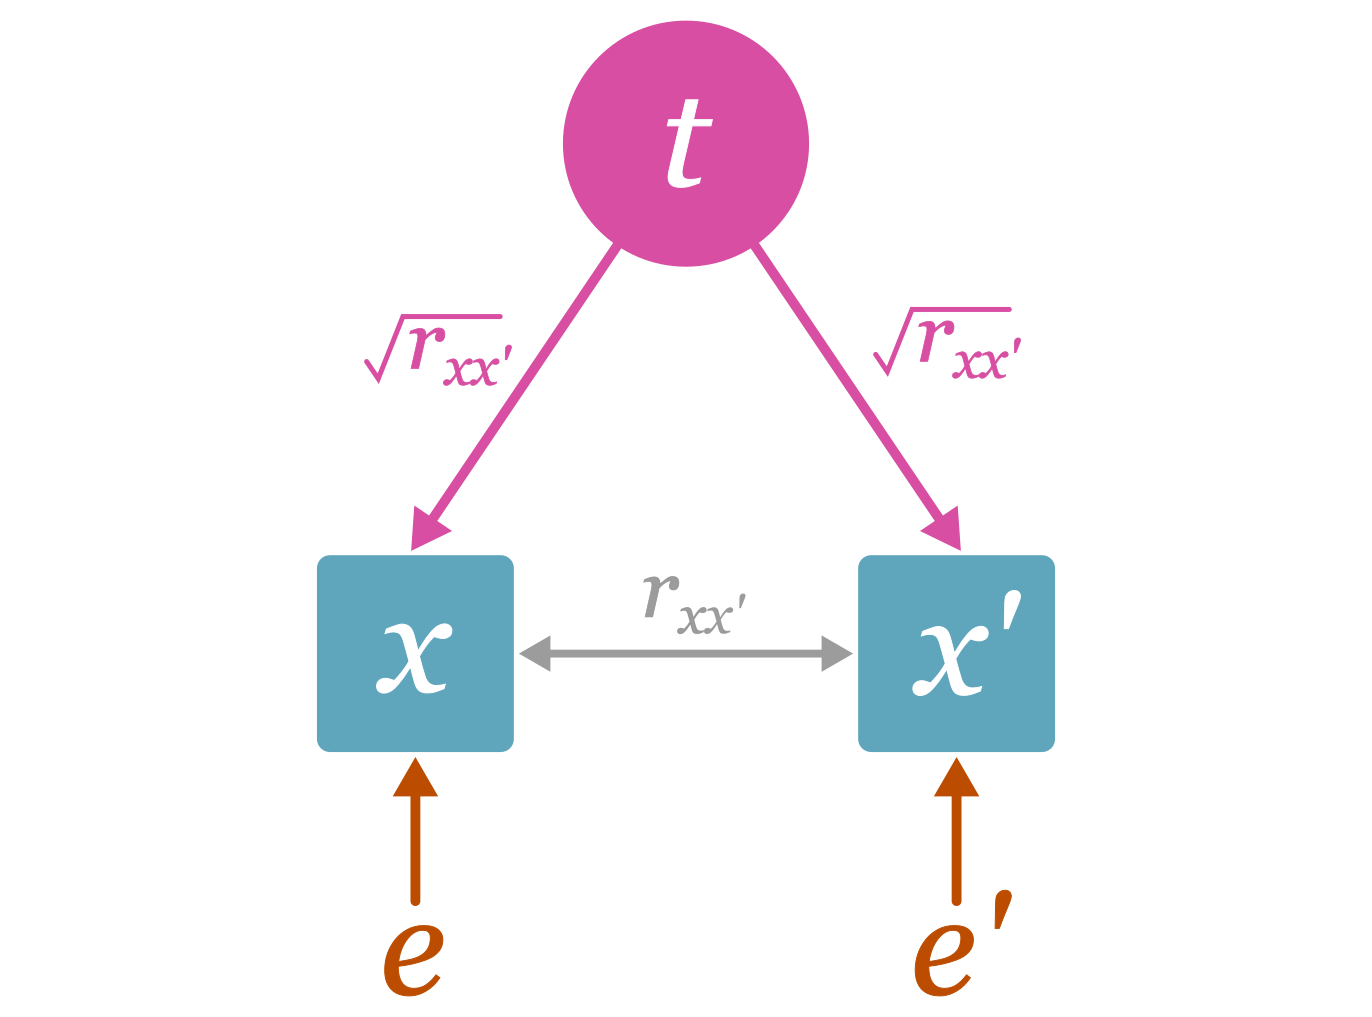
\includegraphics[width=4.16667in,height=\textheight]{figure/unreliability_diagram_1.png}

}

\caption{Structural model illustrating the relationship between true
scores, observed scores, and error scores. The pink circle labeled \(t\)
indicates the true scores, the blue squares labeled with \(x\) and
\(x'\) represent observed scores on parallel measurements, and the red
\(e\) denotes error. Correlations between \(t\), \(x\), and \(x'\) are
in terms of reliability (\(r_{xx'}\)). Note that
\(\sqrt{r_{xx'}}=r_{xt}\).}

\end{figure}

Given that errors do not co-vary between parallel measurements and true
scores are held constant over measurements, it becomes apparent that the
covariance between observed scores produced from parallel measurements
must solely be attributable to true score variance,
\(\sigma_{xx'}=\sigma_t^2\). The covariance in observed scores can be
standardized to obtain the correlation coefficient between parallel
measurements (i.e., the reliability), such that,

\[r_{xx'}=\frac{\sigma_{xx'}}{\sigma_x\sigma_{x'}}  = \frac{\sigma_t^2}{\sigma^2_{x}}\]

Therefore reliability can be expressed in a few forms different forms

\begin{equation}\protect\hypertarget{eq-reliability}{}{
r_{xx'} =r^2_{xt} = \frac{\sigma_t^2}{\sigma_t^2+\sigma_{e}^2} = \frac{\sigma_t^2}{\sigma_{x}^2}
}\label{eq-reliability}\end{equation}

In the literature, the correlation between observed and true scores,
\(r_{xt}\), is often referred to as the ``measure quality index'' (John
E. Hunter and Schmidt 1990), however measure quality encompasses both
reliability \emph{and} validity. Validity A measure can demonstrate high
reliability even though the scores produced by the measure do not
accurately reflect the measurand (the quantity that we are intending to
measure). For example, if an individual were to step on a weight scale
with shoes on, the weight presented on the scale would be highly
reliable, namely, if the individual were to repeat this process, they
would achieve highly similar results. Nevertheless, the observed weight
is systematically biased upward by the weight of the shoes. Therefore if
a measure is reliable it does not logically follow that the measure is
necessarily valid.

\hypertarget{estimating-reliability}{%
\section{Estimating Reliability}\label{estimating-reliability}}

In practice, reliability must be estimated through indirect methods,
since true scores and errors are unknown. Their are many estimators that
can be used however, we will go over three of the most common
approaches: coefficient alpha, split-half, and test-retest reliability.

\hypertarget{internal-consistency-estimators}{%
\subsection*{Internal Consistency
Estimators}\label{internal-consistency-estimators}}
\addcontentsline{toc}{subsection}{Internal Consistency Estimators}

Maybe the most conventionally reported reliability estimator in the
psychological sciences is coefficient alpha, also referred to as
Cronbach's alpha or internal consistency. Alpha has the benefit of being
computationally convenient, but it also brings along many assumptions
that are often violated in practice (Haertel 2006; Sijtsma 2009).
Cronbach's alpha, along with other internal consistency estimators,
serves the purpose of assessing the reliability of composite measures
comprising multiple components. Taking multiple measurements and then
averaging tends to provide a better estimate of true values. For
instance, let's consider the case of Francis Galton (Galton 1907), who
conducted a study involving 787 individuals estimating the weight of an
ox. On average, each person's estimate deviated by approximately 37
pounds from the actual weight of the ox, which was recorded as 1198
pounds. However, when all the guesses were averaged together, the
combined estimate was 1207 pounds, just a 9 pound difference from the
actual value. Averaging a number of noisy estimates provides a much more
stable and reliable estimate. So to create a more stable composite score
(\(X\)), we can take the score (\(x_m\)) from \(k\) measurements and
average them such that, \[
X = \frac{1}{k}(x_1 + x_2 +...+x_k)= \frac{1}{k}\sum^k_{m=1}x_m
\] Coefficient alpha is represents the reliability of this composite
scores. Coefficient alpha only requires three parameters to calculate,
the number of measurements (\(k\)), the variances of each items (
\(\sigma^2_{x_m}\)), and the variance of the composite score
(\(\sigma^2_{X}\)),

\[
_\alpha r_{X X'} = \frac{k}{k-1}\left( 1 - \frac{\sum_{m=1}^k \sigma^2_{x_m}}{\sigma^2_{X}} \right)
\]

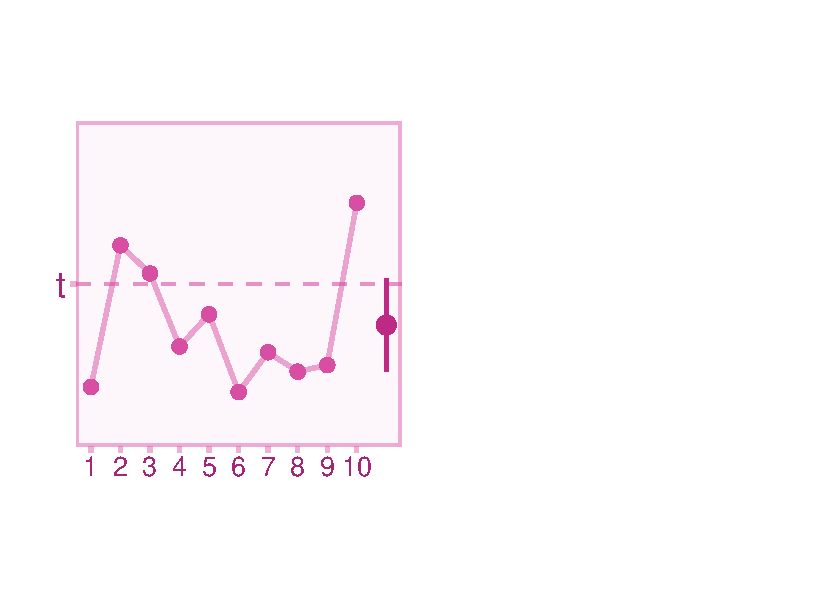
\includegraphics{unreliability_files/figure-pdf/unnamed-chunk-1-1.pdf}

With tighter assumptions (i.e., strictly parallel forms, Haertel 2006),
the formula for coefficient alpha can be simplified to just two
parameters: the number of measurements and the average correlation
between measured scores (\(\bar{r}_{x_i x_j}\), where \(i\neq j\)). This
formula is known as Spearman-Brown's prophecy,

\[
_\text{sb} r_{XX'}= \frac{k \bar{r}_{x_i x_j}}{1+(k-1)\bar{r}_{x_i x_j}}
\]

This can be simplified further if we we have two observed scores. This
formulation is traditionally called split-half reliability:

\[
_\text{sh}r_{XX',}= \frac{2r_{x_1 x_2}}{1+r_{x_1 x_2}}
\]

All of these reliability estimators measure internal consistency,
therefore they do not account for error outside of the
measurement-specific error. There are other sources of error that
internal consistency reliability estimates do not account for, such as
transient error or rater-specific error.

\begin{figure}

{\centering 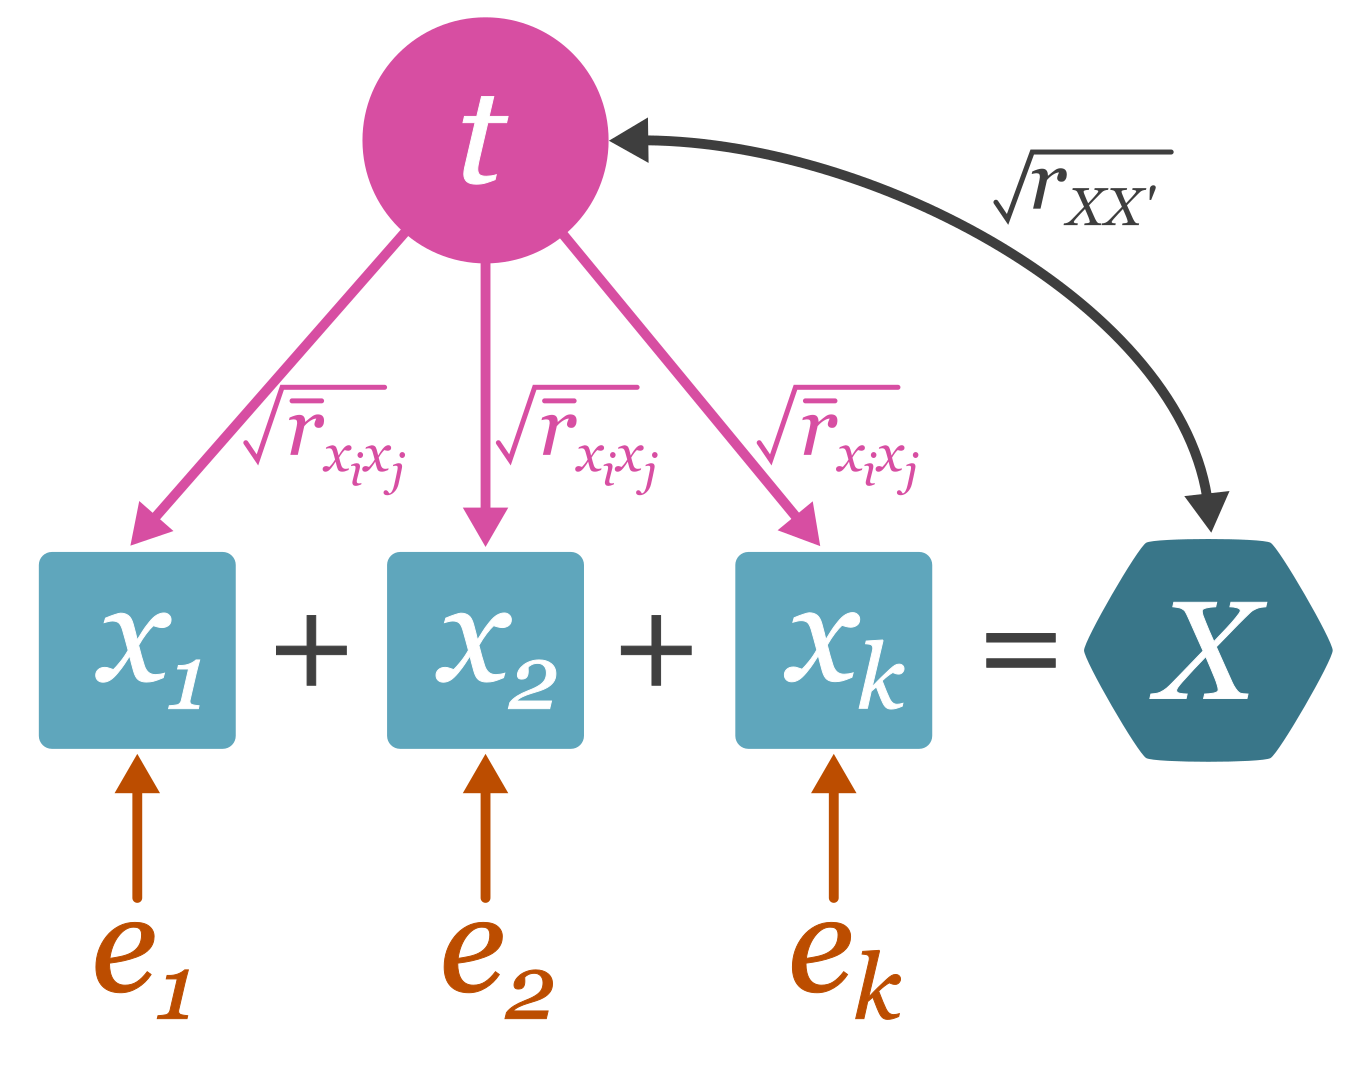
\includegraphics[width=4.16667in,height=\textheight]{figure/unreliability_diagram_2.png}

}

\caption{Structural model illustrating internal consistency. The pink
circle labeled \(t\) indicates the true scores, the blue squares,
\(x_{1...k}\), represent the observed scores across multiple
measurements, and the red \(e\) denotes error. The dark blue hexagon,
\(X\), indicates a composite score as a sum of the observed scores
(\(x_{1...k}\)). Note that \(\sqrt{r_{XX'}}=r_{Xt}\).}

\end{figure}

\hypertarget{calculating-internal-consistency-in-r-and-python}{%
\subsubsection*{Calculating Internal Consistency in R and
Python}\label{calculating-internal-consistency-in-r-and-python}}
\addcontentsline{toc}{subsubsection}{Calculating Internal Consistency in
R and Python}

\subsubsection{R}

Let us simulate a data set of 50 individuals where each observed score
has the same true score with some error.

\begin{Shaded}
\begin{Highlighting}[]
\CommentTok{\#set seed}
\FunctionTok{set.seed}\NormalTok{(}\DecValTok{343}\NormalTok{)}

\CommentTok{\# set sample size}
\NormalTok{n }\OtherTok{=} \DecValTok{50}

\CommentTok{\# simulate data}
\NormalTok{t }\OtherTok{=} \FunctionTok{rnorm}\NormalTok{(n, }\DecValTok{0}\NormalTok{, }\DecValTok{1}\NormalTok{) }\CommentTok{\# simulate true scores}
\NormalTok{x1 }\OtherTok{=}\NormalTok{ t }\SpecialCharTok{+} \FunctionTok{rnorm}\NormalTok{(n, }\DecValTok{0}\NormalTok{, }\DecValTok{1}\NormalTok{) }\CommentTok{\# simulate observed scores for measurement 1}
\NormalTok{x2 }\OtherTok{=}\NormalTok{ t }\SpecialCharTok{+} \FunctionTok{rnorm}\NormalTok{(n, }\DecValTok{0}\NormalTok{, }\DecValTok{1}\NormalTok{) }\CommentTok{\# simulate observed scores for measurement 2}
\NormalTok{x3 }\OtherTok{=}\NormalTok{ t }\SpecialCharTok{+} \FunctionTok{rnorm}\NormalTok{(n, }\DecValTok{0}\NormalTok{, }\DecValTok{1}\NormalTok{) }\CommentTok{\# simulate observed scores for measurement 3}
\NormalTok{x4 }\OtherTok{=}\NormalTok{ t }\SpecialCharTok{+} \FunctionTok{rnorm}\NormalTok{(n, }\DecValTok{0}\NormalTok{, }\DecValTok{1}\NormalTok{) }\CommentTok{\# simulate observed scores for measurement 4}

\CommentTok{\# calculate composite score}
\NormalTok{X }\OtherTok{=}\NormalTok{ x1 }\SpecialCharTok{+}\NormalTok{ x2 }\SpecialCharTok{+}\NormalTok{ x3 }\SpecialCharTok{+}\NormalTok{ x4}
\end{Highlighting}
\end{Shaded}

Calculate Coefficient Alpha Reliability:

\begin{Shaded}
\begin{Highlighting}[]
\CommentTok{\# step 1. calculate variance of observed (measured) scores}
\NormalTok{var\_xi }\OtherTok{=} \FunctionTok{c}\NormalTok{(}\FunctionTok{var}\NormalTok{(x1),}\FunctionTok{var}\NormalTok{(x2),}\FunctionTok{var}\NormalTok{(x3),}\FunctionTok{var}\NormalTok{(x4))}

\CommentTok{\# step 2. calculate variance of composite score}
\NormalTok{var\_X }\OtherTok{=} \FunctionTok{var}\NormalTok{(X)}

\CommentTok{\# step 3. get number of items (k)}
\NormalTok{k }\OtherTok{=} \FunctionTok{length}\NormalTok{(var\_xi)}

\CommentTok{\# step 4. calculate coefficient alpha reliability}
\NormalTok{rXX\_alpha }\OtherTok{=}\NormalTok{ k }\SpecialCharTok{/}\NormalTok{ (k}\DecValTok{{-}1}\NormalTok{) }\SpecialCharTok{*}\NormalTok{ (}\DecValTok{1} \SpecialCharTok{{-}} \FunctionTok{sum}\NormalTok{(var\_xi)}\SpecialCharTok{/}\NormalTok{var\_X)}

\CommentTok{\# display reliability}
\FunctionTok{print}\NormalTok{(}\FunctionTok{round}\NormalTok{(rXX\_alpha,}\DecValTok{3}\NormalTok{)) }
\end{Highlighting}
\end{Shaded}

\begin{verbatim}
[1] 0.775
\end{verbatim}

Calculate Reliability via Spearman-Brown's Prophecy:

\begin{Shaded}
\begin{Highlighting}[]
\CommentTok{\# step 1. get correlation matrix between all observed scores}
\NormalTok{corr\_mat }\OtherTok{=} \FunctionTok{cor}\NormalTok{(}\FunctionTok{cbind}\NormalTok{(x1,x2,x3,x4))}

\CommentTok{\# step 2. average off{-}diagonal elements of matrix}
\FunctionTok{diag}\NormalTok{(corr\_mat) }\OtherTok{\textless{}{-}} \ConstantTok{NA}
\NormalTok{rxixj }\OtherTok{=} \FunctionTok{mean}\NormalTok{(corr\_mat, }\AttributeTok{na.rm =} \ConstantTok{TRUE}\NormalTok{)}

\CommentTok{\# step 3. get number of items (k)}
\NormalTok{k }\OtherTok{=} \FunctionTok{dim}\NormalTok{(corr\_mat)[}\DecValTok{1}\NormalTok{]}

\CommentTok{\# step 4. calculate Spearman{-}Brown reliability}
\NormalTok{rXX\_SB }\OtherTok{=}\NormalTok{ k }\SpecialCharTok{*}\NormalTok{ rxixj }\SpecialCharTok{/}\NormalTok{ (}\DecValTok{1} \SpecialCharTok{+}\NormalTok{ (k}\DecValTok{{-}1}\NormalTok{) }\SpecialCharTok{*}\NormalTok{ rxixj)}

\CommentTok{\# display reliability}
\FunctionTok{print}\NormalTok{(}\FunctionTok{round}\NormalTok{(rXX\_SB,}\DecValTok{3}\NormalTok{)) }
\end{Highlighting}
\end{Shaded}

\begin{verbatim}
[1] 0.775
\end{verbatim}

Calculate the Split-Half Reliability:

\begin{Shaded}
\begin{Highlighting}[]
\CommentTok{\# step 1. make composite scores for each half of the observed scores}
\NormalTok{X1 }\OtherTok{=}\NormalTok{ x1 }\SpecialCharTok{+}\NormalTok{ x2}
\NormalTok{X2 }\OtherTok{=}\NormalTok{ x3 }\SpecialCharTok{+}\NormalTok{ x4}

\CommentTok{\# step 2. calculate the correlation between the scores of both halves}
\NormalTok{rX1X2 }\OtherTok{=} \FunctionTok{cor}\NormalTok{(X1,X2)}

\CommentTok{\# step 3. calculate the split{-}half reliability}
\NormalTok{rXX\_SH }\OtherTok{=} \DecValTok{2}\SpecialCharTok{*}\NormalTok{rX1X2 }\SpecialCharTok{/}\NormalTok{ (}\DecValTok{1} \SpecialCharTok{+}\NormalTok{ rX1X2)}

\CommentTok{\# display reliability}
\FunctionTok{print}\NormalTok{(}\FunctionTok{round}\NormalTok{(rXX\_SH,}\DecValTok{3}\NormalTok{)) }
\end{Highlighting}
\end{Shaded}

\begin{verbatim}
[1] 0.824
\end{verbatim}

True Reliability: Lets see how the results compare to the squared
correlation of the true scores and our composite score (true
reliability).

\begin{Shaded}
\begin{Highlighting}[]
\CommentTok{\# calculate true reliability}
\NormalTok{rXt }\OtherTok{=} \FunctionTok{cor}\NormalTok{(X,t)}

\CommentTok{\# display true reliability}
\FunctionTok{print}\NormalTok{(}\FunctionTok{round}\NormalTok{(rXt}\SpecialCharTok{\^{}}\DecValTok{2}\NormalTok{,}\DecValTok{3}\NormalTok{)) }
\end{Highlighting}
\end{Shaded}

\begin{verbatim}
[1] 0.753
\end{verbatim}

In this case, the reliability estimates do a fairly good job of
estimating the true reliability of the observed scores.

\subsubsection{Python}

Simulate Data: Let us simulate a data set of 50 individuals where each
observed score has the same true score with some error. To calculate the
necessary statistics, we will import the \texttt{numpy} package.

\begin{Shaded}
\begin{Highlighting}[]
\CommentTok{\#import numpy}
\ImportTok{import}\NormalTok{ numpy }\ImportTok{as}\NormalTok{ np}

\CommentTok{\# set seed}
\NormalTok{np.random.seed(}\DecValTok{343}\NormalTok{)}

\CommentTok{\# set sample size}
\NormalTok{n }\OperatorTok{=} \DecValTok{50}

\CommentTok{\# simulate data}
\NormalTok{t }\OperatorTok{=}\NormalTok{ np.random.normal(}\DecValTok{0}\NormalTok{, }\DecValTok{1}\NormalTok{, n) }\CommentTok{\# simulate true scores}
\NormalTok{x1 }\OperatorTok{=}\NormalTok{ t }\OperatorTok{+}\NormalTok{ np.random.normal(}\DecValTok{0}\NormalTok{, }\DecValTok{1}\NormalTok{, n) }\CommentTok{\# simulate observed scores for measurement 1}
\NormalTok{x2 }\OperatorTok{=}\NormalTok{ t }\OperatorTok{+}\NormalTok{ np.random.normal(}\DecValTok{0}\NormalTok{, }\DecValTok{1}\NormalTok{, n) }\CommentTok{\# simulate observed scores for measurement 2}
\NormalTok{x3 }\OperatorTok{=}\NormalTok{ t }\OperatorTok{+}\NormalTok{ np.random.normal(}\DecValTok{0}\NormalTok{, }\DecValTok{1}\NormalTok{, n) }\CommentTok{\# simulate observed scores for measurement 3}
\NormalTok{x4 }\OperatorTok{=}\NormalTok{ t }\OperatorTok{+}\NormalTok{ np.random.normal(}\DecValTok{0}\NormalTok{, }\DecValTok{1}\NormalTok{, n) }\CommentTok{\# simulate observed scores for measurement 4}

\CommentTok{\# calculate sum score}
\NormalTok{X }\OperatorTok{=}\NormalTok{ x1 }\OperatorTok{+}\NormalTok{ x2 }\OperatorTok{+}\NormalTok{ x3 }\OperatorTok{+}\NormalTok{ x4}
\end{Highlighting}
\end{Shaded}

Calculate Coefficient Alpha Reliability:

\begin{Shaded}
\begin{Highlighting}[]
\CommentTok{\# step 1. calculate variance of observed (measured) scores}
\NormalTok{var\_xm }\OperatorTok{=}\NormalTok{ [np.var(x1),np.var(x2),np.var(x3),np.var(x4)]}

\CommentTok{\# step 2. calculate variance of composite score}
\NormalTok{var\_X }\OperatorTok{=}\NormalTok{ np.var(X)}

\CommentTok{\# step 3. get number of items (k)}
\NormalTok{k }\OperatorTok{=} \BuiltInTok{len}\NormalTok{(var\_xm)}

\CommentTok{\# step 4. calculate coefficient alpha reliability}
\NormalTok{rXX\_alpha }\OperatorTok{=}\NormalTok{ k }\OperatorTok{/}\NormalTok{ (k}\OperatorTok{{-}}\DecValTok{1}\NormalTok{) }\OperatorTok{*}\NormalTok{ (}\DecValTok{1} \OperatorTok{{-}} \BuiltInTok{sum}\NormalTok{(var\_xm)}\OperatorTok{/}\NormalTok{var\_X)}

\BuiltInTok{print}\NormalTok{(}\BuiltInTok{round}\NormalTok{(rXX\_alpha,}\DecValTok{3}\NormalTok{)) }
\end{Highlighting}
\end{Shaded}

\begin{verbatim}
0.769
\end{verbatim}

Calculate Reliability from Spearman-Brown's prophecy formula:

\begin{Shaded}
\begin{Highlighting}[]
\CommentTok{\# step 1. get correlation matrix between all observed scores}
\NormalTok{corr\_mat }\OperatorTok{=}\NormalTok{ np.corrcoef([x1,x2,x3,x4])}

\CommentTok{\# step 2. average off{-}diagonal elements of matrix}
\NormalTok{rxixj }\OperatorTok{=}\NormalTok{ np.mean(corr\_mat[}\OperatorTok{\textasciitilde{}}\NormalTok{np.eye(k,dtype}\OperatorTok{=}\BuiltInTok{bool}\NormalTok{)])}

\CommentTok{\# step 3. get number of items (k)}
\NormalTok{k }\OperatorTok{=} \BuiltInTok{len}\NormalTok{(corr\_mat)}

\CommentTok{\# step 4. calculate Spearman{-}Brown reliability}
\NormalTok{rXX\_SB }\OperatorTok{=}\NormalTok{ k }\OperatorTok{*}\NormalTok{ rxixj }\OperatorTok{/}\NormalTok{ (}\DecValTok{1} \OperatorTok{+}\NormalTok{ (k}\OperatorTok{{-}}\DecValTok{1}\NormalTok{) }\OperatorTok{*}\NormalTok{ rxixj)}

\BuiltInTok{print}\NormalTok{(}\BuiltInTok{round}\NormalTok{(rXX\_SB,}\DecValTok{3}\NormalTok{)) }
\end{Highlighting}
\end{Shaded}

\begin{verbatim}
0.772
\end{verbatim}

Calculate Split-Half Reliability:

\begin{Shaded}
\begin{Highlighting}[]
\CommentTok{\# step 1. make composite scores for each half of the observed scores}
\NormalTok{X1 }\OperatorTok{=}\NormalTok{ x1 }\OperatorTok{+}\NormalTok{ x2}
\NormalTok{X2 }\OperatorTok{=}\NormalTok{ x3 }\OperatorTok{+}\NormalTok{ x4}

\CommentTok{\# step 2. calculate the correlation between the scores of both halves}
\NormalTok{rX1X2 }\OperatorTok{=}\NormalTok{ np.corrcoef(X1,X2)[}\DecValTok{0}\NormalTok{,}\DecValTok{1}\NormalTok{]}

\CommentTok{\# step 3. calculate the split{-}half reliability}
\NormalTok{rXX\_SH }\OperatorTok{=} \DecValTok{2}\OperatorTok{*}\NormalTok{rX1X2 }\OperatorTok{/}\NormalTok{ (}\DecValTok{1} \OperatorTok{+}\NormalTok{ rX1X2)}

\CommentTok{\# display reliability}
\BuiltInTok{print}\NormalTok{(}\BuiltInTok{round}\NormalTok{(rXX\_SH,}\DecValTok{3}\NormalTok{)) }
\end{Highlighting}
\end{Shaded}

\begin{verbatim}
0.772
\end{verbatim}

Lets see how the results compare to the squared correlation of the true
scores and our composite score (true reliability).

\begin{Shaded}
\begin{Highlighting}[]
\CommentTok{\# calculate true reliability}
\NormalTok{rXt }\OperatorTok{=}\NormalTok{ np.corrcoef(X,t)[}\DecValTok{0}\NormalTok{,}\DecValTok{1}\NormalTok{]}

\CommentTok{\# display reliability}
\BuiltInTok{print}\NormalTok{(}\BuiltInTok{round}\NormalTok{(rXt}\OperatorTok{**}\DecValTok{2}\NormalTok{,}\DecValTok{3}\NormalTok{)) }
\end{Highlighting}
\end{Shaded}

\begin{verbatim}
0.791
\end{verbatim}

In this case, the reliability estimates do a fairly good job of
estimating the true reliability of the observed scores. There are also
functions within the \texttt{psych} package that allow you to easily
calculate coefficient alpha among other reliability estimators

\hypertarget{test-retest-stability-estimator}{%
\subsection{Test-Retest Stability
Estimator}\label{test-retest-stability-estimator}}

There measurement errors that exist outside of the measurement
instrument itself. Transient errors represent fluctuations in observed
scores over time. These fluctuations, even if they are systematic (e.g.,
fatigue over the course of a single day), add extraneous within-person
variance that can mask true scores (i.e., expectation of observed
scores). For example, if a researcher wants to investigate how
individuals differ in processing speed, then variation within an
individual's scores across multiple testing sessions would be considered
error since the goal of the study is to investigate between-person
variation. Considering transient fluctuations as error depends on the
research goal, so it is important for researchers to take care in
considering which variance components should be considered error in
their study. To estimate test-retest reliability, we can compute the
pearson correlation coefficient between the measurement at time 1
(\(x_{T_{1}}\)) and the second measurement at time 2 (\(x_{T_{2}}\)).

\[
_\text{tr}r_{xx'}= r_{x_{T_1}x_{T_2}}
\]

Note that calculating the pearson correlation coefficient between
time-points ignores systematic changes (e.g., practice effects).

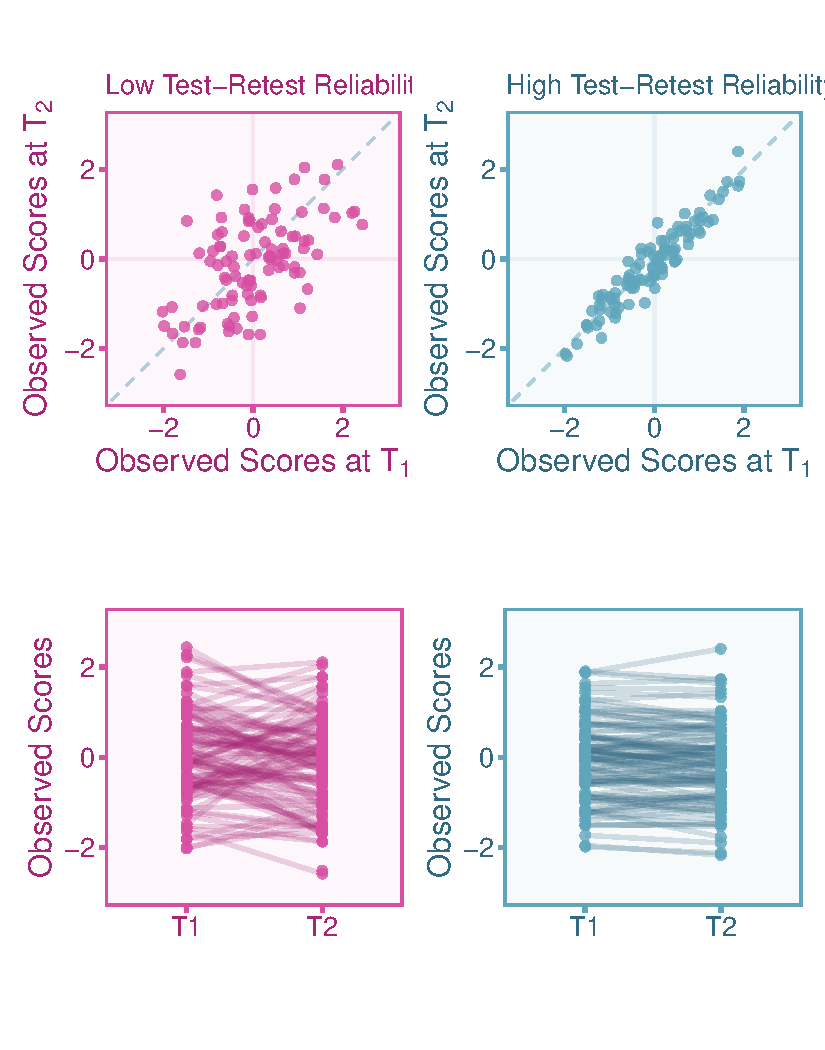
\includegraphics{unreliability_files/figure-pdf/unnamed-chunk-12-1.pdf}

\hypertarget{calculating-test-retest-reliability-in-r-and-python}{%
\subsubsection*{Calculating Test-Retest Reliability in R and
Python}\label{calculating-test-retest-reliability-in-r-and-python}}
\addcontentsline{toc}{subsubsection}{Calculating Test-Retest Reliability
in R and Python}

\subsubsection{R}

Lets calculate test-retest reliability in R. First, we can simulate
observed scores at two time points, \(T_1\) and \(T_2\). We can assume
that the true scores remain constant between \(T_1\) and \(T_2\).
Second, we can calculate the correlation between the observed scores at
each time point (\(r_{x_{T_1}x_{T_2}}\)).

\begin{Shaded}
\begin{Highlighting}[]
\CommentTok{\# set seed}
\FunctionTok{set.seed}\NormalTok{(}\DecValTok{343}\NormalTok{)}

\CommentTok{\# set sample size}
\NormalTok{n }\OtherTok{=} \DecValTok{70}

\CommentTok{\# simulate true scores}
\NormalTok{t }\OtherTok{=} \FunctionTok{rnorm}\NormalTok{(n,}\DecValTok{0}\NormalTok{,}\DecValTok{1}\NormalTok{)}

\CommentTok{\# simulate scores at time 1}
\NormalTok{xT1 }\OtherTok{=}\NormalTok{ t }\SpecialCharTok{+} \FunctionTok{rnorm}\NormalTok{(n,}\DecValTok{0}\NormalTok{,.}\DecValTok{5}\NormalTok{)}

\CommentTok{\# simulate scores at time 2}
\NormalTok{xT2 }\OtherTok{=}\NormalTok{ t }\SpecialCharTok{+} \FunctionTok{rnorm}\NormalTok{(n,}\DecValTok{0}\NormalTok{,.}\DecValTok{5}\NormalTok{)}

\CommentTok{\# calculate test{-}retest reliability}
\NormalTok{rxx }\OtherTok{=} \FunctionTok{cor}\NormalTok{(xT1,xT2)}

\CommentTok{\# display reliability}
\FunctionTok{print}\NormalTok{(}\FunctionTok{round}\NormalTok{(rxx,}\DecValTok{3}\NormalTok{))}
\end{Highlighting}
\end{Shaded}

\begin{verbatim}
[1] 0.803
\end{verbatim}

\begin{Shaded}
\begin{Highlighting}[]
\CommentTok{\# compare with true reliability}
\NormalTok{rxx\_true }\OtherTok{=} \FunctionTok{cor}\NormalTok{(xT1,t)}\SpecialCharTok{\^{}}\DecValTok{2}

\CommentTok{\# display true reliability}
\FunctionTok{print}\NormalTok{(}\FunctionTok{round}\NormalTok{(rxx\_true,}\DecValTok{3}\NormalTok{))}
\end{Highlighting}
\end{Shaded}

\begin{verbatim}
[1] 0.768
\end{verbatim}

\subsubsection{Python}

Lets calculate test-retest reliability in R. First, we can simulate
observed scores at two time points, \(T_1\) and \(T_2\). We can assume
that the true scores remain constant between \(T_1\) and \(T_2\).
Second, we can calculate the correlation between the observed scores at
each time point (\(r_{x_{T_1}x_{T_2}}\)).

\begin{Shaded}
\begin{Highlighting}[]
\CommentTok{\# import numpy}
\ImportTok{import}\NormalTok{ numpy }\ImportTok{as}\NormalTok{ np}

\CommentTok{\# set seed}
\NormalTok{np.random.seed(}\DecValTok{343}\NormalTok{)}

\CommentTok{\# set sample size}
\NormalTok{n }\OperatorTok{=} \DecValTok{70}

\CommentTok{\# simulate 70 true scores}
\NormalTok{t }\OperatorTok{=}\NormalTok{ np.random.normal(}\DecValTok{0}\NormalTok{,}\DecValTok{1}\NormalTok{,n)}

\CommentTok{\# simulate scores at time 1}
\NormalTok{xT1 }\OperatorTok{=}\NormalTok{ t }\OperatorTok{+}\NormalTok{ np.random.normal(}\DecValTok{0}\NormalTok{,}\FloatTok{.5}\NormalTok{,n)}

\CommentTok{\# simulate scores at time 2}
\NormalTok{xT2 }\OperatorTok{=}\NormalTok{ t }\OperatorTok{+}\NormalTok{ np.random.normal(}\DecValTok{0}\NormalTok{,}\FloatTok{.5}\NormalTok{,n)}

\CommentTok{\# calculate test{-}retest reliability}
\NormalTok{rxx }\OperatorTok{=}\NormalTok{ np.corrcoef(xT1,xT2)[}\DecValTok{0}\NormalTok{,}\DecValTok{1}\NormalTok{]}

\CommentTok{\# display reliability}
\BuiltInTok{print}\NormalTok{(}\BuiltInTok{round}\NormalTok{(rxx,}\DecValTok{3}\NormalTok{))}
\end{Highlighting}
\end{Shaded}

\begin{verbatim}
0.768
\end{verbatim}

\begin{Shaded}
\begin{Highlighting}[]
\CommentTok{\# compare with true reliability}
\NormalTok{rxx\_true }\OperatorTok{=}\NormalTok{ np.corrcoef(xT1,t)[}\DecValTok{0}\NormalTok{,}\DecValTok{1}\NormalTok{]}\OperatorTok{**}\DecValTok{2}

\CommentTok{\# display true reliability}
\BuiltInTok{print}\NormalTok{(}\BuiltInTok{round}\NormalTok{(rxx\_true,}\DecValTok{3}\NormalTok{))}
\end{Highlighting}
\end{Shaded}

\begin{verbatim}
0.731
\end{verbatim}

\hypertarget{sources-of-measurement-error}{%
\subsection{Sources of Measurement
Error}\label{sources-of-measurement-error}}

There are many estimators of reliability beyond internal consistency and
test-retest that account for different sources of error and hold
different assumptions. There are many sources of measurement error that
different estimators of reliability account for adapted from table 1 of
Wiernik and Dahlke (2020) :

\begin{itemize}
\item
  Random Response Error: Genuine randomness in responses. Examples
  include: motor errors and variation in response time.
\item
  Time/Environment-Specific (Transient) Error: Fluctuations in scores as
  a result of the specific time or environment of the measurement. For
  instance, if researchers administered an ability test to a sample of
  undergraduate students throughout the course of a day, the student's
  who complete the test at the end of the day will likely perform worse
  than participant's who completed due to fatigue rather than ability.
  Errors due to illness, mood, hunger, environmental distractors, etc.
  all fall under the umbrella of transient errors.
\item
  Instrument-Specific Error: Error due to the specific content or
  make-up of the measurement instrument. For example, a psychological
  scale using likert items participant's idiosyncratic interpretations
  of questions and response options rather than their standing on the
  latent construct.
\item
  Rater/Observer-Specific Error: Errors induced by idiosyncratic biases
  of individual raters and rater by ratee interactions (e.g., Teacher A
  gives higher grades to students who stay after class).
\end{itemize}

Different estimators of reliability account for different sources of
measurement error therefore depending on the research design, it is
important to carefully choose which reliability is most relevant for
your use case. Note that even if two estimators account for the same
types of measurement error, they likely hold different assumptions that
may be violated in a given research context.

\begin{longtable}[]{@{}
  >{\raggedright\arraybackslash}p{(\columnwidth - 10\tabcolsep) * \real{0.1644}}
  >{\raggedright\arraybackslash}p{(\columnwidth - 10\tabcolsep) * \real{0.1781}}
  >{\centering\arraybackslash}p{(\columnwidth - 10\tabcolsep) * \real{0.1644}}
  >{\centering\arraybackslash}p{(\columnwidth - 10\tabcolsep) * \real{0.1644}}
  >{\centering\arraybackslash}p{(\columnwidth - 10\tabcolsep) * \real{0.1644}}
  >{\centering\arraybackslash}p{(\columnwidth - 10\tabcolsep) * \real{0.1644}}@{}}
\caption{Table 1. List of reliability coefficients and the sources of
error they account for.}\tabularnewline
\toprule\noalign{}
\begin{minipage}[b]{\linewidth}\raggedright
Estimator
\end{minipage} & \begin{minipage}[b]{\linewidth}\raggedright
Description
\end{minipage} & \begin{minipage}[b]{\linewidth}\centering
Random Response Error
\end{minipage} & \begin{minipage}[b]{\linewidth}\centering
Transient Error
\end{minipage} & \begin{minipage}[b]{\linewidth}\centering
Instrument-Specific Error
\end{minipage} & \begin{minipage}[b]{\linewidth}\centering
Rater-Specific Error
\end{minipage} \\
\midrule\noalign{}
\endfirsthead
\toprule\noalign{}
\begin{minipage}[b]{\linewidth}\raggedright
Estimator
\end{minipage} & \begin{minipage}[b]{\linewidth}\raggedright
Description
\end{minipage} & \begin{minipage}[b]{\linewidth}\centering
Random Response Error
\end{minipage} & \begin{minipage}[b]{\linewidth}\centering
Transient Error
\end{minipage} & \begin{minipage}[b]{\linewidth}\centering
Instrument-Specific Error
\end{minipage} & \begin{minipage}[b]{\linewidth}\centering
Rater-Specific Error
\end{minipage} \\
\midrule\noalign{}
\endhead
\bottomrule\noalign{}
\endlastfoot
Coefficient Alpha & Internal consistency coefficient for composite
measures. & ✔️ & & ✔️ & \\
Coefficient Omega & Internal consistency coefficient for composite
measures with specified factor structure. & ✔️ & & ✔️ & \\
Split-Half & Internal consistency coefficient for measurements that are
split into two halves. & ✔️ & & ✔️ & \\
Kuder-Richardson 20 & Internal consistency when observed scores are
binary (special case of coefficient alpha). & ✔️ & & ✔️ & \\
Item Response Theory Reliability & Reliability coefficient derived from
item response theory (as opposed to classical test theory) & ✔️ & & ✔️
& \\
Inter-Rater/Inter-Observer Reliability & Consistency in scoring between
raters/observers. & ✔️ & & & ✔️ \\
Test-Retest & Stability coefficient for repeated measurements across
time & ✔️ & ✔️ & & \\
Delayed Coefficient Alpha & Average of all possible split-half
reliabilities & ✔️ & ✔️ & ✔️ & \\
G-Coefficient & Reliability coefficient derived from generalizability
theory (G-theory). Can incorporate any source of error if enough data is
present. & ✔️ & ✔️ & ✔️ & ✔️ \\
\end{longtable}

\hypertarget{bias-in-correlation-coefficients}{%
\section{Bias in Correlation
Coefficients}\label{bias-in-correlation-coefficients}}

Unreliability induces systematic bias in effect size estimates such as
correlation coefficients Spearman (1904). Lets say we have two observed
scores \$x\$ and \$y\$,

\[
x=x_t+e
\]

\[
y=y_t+e
\]

In most research contexts, we would like to estimate the correlation
between true scores where the correlation between true scores, \(x_t\)
and \(y_t\) is \[
\rho=\frac{\sigma_{x_ty_t}}{\sigma_{x_t} \sigma_{y_t}}
\]

The observed correlation differs only in that it standardizes the
covariance by the product of the standard deviations of observed scores
rather than true scores. The covariance of observed scores will be
equivalent to the covariance of true scores assuming
\(\sigma_{e_x e_y}=0\) (see Section~\ref{sec-true-score-theory}).

\begin{equation}\protect\hypertarget{eq-bias}{}{
r=\frac{\sigma_{xy}}{\sigma_x \sigma_y} = \frac{\sigma_{x_ty_t}}{\sigma_x \sigma_y}
}\label{eq-bias}\end{equation}

In the presence of measurement error, the observed standard deviations
(\(\sigma_x\) and \(\sigma_y\)) will be larger than the true standard
deviations (\(\sigma_x\) and \(\sigma_y\)). Since the reliability is
defined as the ratio of true variance to total observed variance (see
Equation~\ref{eq-reliability} ), we can see how reliability inflates the
true standard deviation

\[
\sigma^2_x =\sigma^2_{x_t} \cdot \frac{\sigma^2_{x}}{\sigma^2_{x_t}} = \sigma^2_{x_t}\cdot\frac{1}{r_{xx'}} = \frac{\sigma^2_{xt}}{r_{xx'}}
\]

Therefore,

\[
\sigma_x = \frac{\sigma_{x_t}}{\sqrt{r_{xx'}}}
\]

If we plug this back into equation Equation~\ref{eq-bias} then we can
see how the observed correlation changes as a function of reliability
and how it is biased from the true score correlation \(\rho\):

\[
\begin{align}
r &= \frac{\sigma_{x_ty_t}}{\sigma_{x} \sigma_{y}} 
\\ &= \frac{\sigma_{x_ty_t}}{\left[\frac{\sigma_{x_t}}{\sqrt{r_{xx'}}} \right] \left[ \frac{\sigma_{y_t}}{\sqrt{r_{yy'}}} \right] } 
\\ &= \frac{\sigma_{x_ty_t}}{\sigma_{x_t}\sigma_{y_t}} \cdot \sqrt{r_{yy'}}\sqrt{r_{xx'}} 
\\ &= \rho\sqrt{r_{yy'}}\sqrt{r_{xx'}}
\end{align}
\] This equation was first provided by Spearman (1904) For cases where
measurement error only affects one of the two variables, the attenuation

\begin{Shaded}
\begin{Highlighting}[]
\NormalTok{rho }\OtherTok{=}\NormalTok{ .}\DecValTok{5}
\NormalTok{X\_true }\OtherTok{=} \FunctionTok{rnorm}\NormalTok{(}\DecValTok{50}\NormalTok{,}\DecValTok{0}\NormalTok{,}\DecValTok{1}\NormalTok{)}
\NormalTok{Y\_true }\OtherTok{=}\NormalTok{ rho }\SpecialCharTok{*}\NormalTok{ X\_true }\SpecialCharTok{+} \FunctionTok{rnorm}\NormalTok{(}\DecValTok{50}\NormalTok{,}\DecValTok{0}\NormalTok{,}\FunctionTok{sqrt}\NormalTok{(}\DecValTok{1}\SpecialCharTok{{-}}\NormalTok{rho}\SpecialCharTok{\^{}}\DecValTok{2}\NormalTok{))}

\NormalTok{h1 }\OtherTok{\textless{}{-}} \FunctionTok{ggplot}\NormalTok{(}\AttributeTok{data =} \ConstantTok{NULL}\NormalTok{, }\FunctionTok{aes}\NormalTok{(}\AttributeTok{x =}\NormalTok{ X\_true, }\AttributeTok{y =}\NormalTok{ Y\_true)) }\SpecialCharTok{+}
    \FunctionTok{geom\_point}\NormalTok{(}\AttributeTok{color =}\NormalTok{ main\_color\_blue, }\AttributeTok{fill =}\NormalTok{ main\_color\_blue) }\SpecialCharTok{+}
    \FunctionTok{scale\_x\_continuous}\NormalTok{(}\AttributeTok{limits =} \FunctionTok{c}\NormalTok{(}\SpecialCharTok{{-}}\DecValTok{3}\NormalTok{,}\DecValTok{3}\NormalTok{)) }\SpecialCharTok{+}
    \FunctionTok{scale\_y\_continuous}\NormalTok{(}\AttributeTok{limits =} \FunctionTok{c}\NormalTok{(}\SpecialCharTok{{-}}\DecValTok{3}\NormalTok{,}\DecValTok{3}\NormalTok{)) }\SpecialCharTok{+}
    \FunctionTok{xlab}\NormalTok{(}\StringTok{"True x"}\NormalTok{)}\SpecialCharTok{+}
    \FunctionTok{ylab}\NormalTok{(}\StringTok{"True y"}\NormalTok{) }\SpecialCharTok{+}
    \FunctionTok{ggtitle}\NormalTok{(}\StringTok{\textquotesingle{}True Score Correlation\textquotesingle{}}\NormalTok{, }\AttributeTok{subtitle =} \FunctionTok{TeX}\NormalTok{(}\StringTok{"$}\SpecialCharTok{\textbackslash{}\textbackslash{}}\StringTok{rho =$ .50"}\NormalTok{)) }\SpecialCharTok{+}
    \FunctionTok{theme}\NormalTok{(}\AttributeTok{aspect.ratio =} \DecValTok{1}\NormalTok{,}
          \AttributeTok{panel.grid.minor =} \FunctionTok{element\_blank}\NormalTok{(),}
          \AttributeTok{panel.grid.major =} \FunctionTok{element\_blank}\NormalTok{(),}
          \AttributeTok{title =} \FunctionTok{element\_text}\NormalTok{(}\AttributeTok{color =}\NormalTok{ text\_color\_blue),}
          \AttributeTok{panel.background =} \FunctionTok{element\_rect}\NormalTok{(}\AttributeTok{fill =}\NormalTok{ panel\_color\_blue),}
          \AttributeTok{panel.border =} \FunctionTok{element\_rect}\NormalTok{(}\AttributeTok{fill =} \ConstantTok{NA}\NormalTok{, }\AttributeTok{color =}\NormalTok{ border\_color\_blue,}\AttributeTok{linewidth=}\FloatTok{1.2}\NormalTok{),}
          \AttributeTok{axis.title =} \FunctionTok{element\_text}\NormalTok{(}\AttributeTok{size=}\DecValTok{14}\NormalTok{, }\AttributeTok{color =}\NormalTok{ text\_color\_blue),}
          \AttributeTok{axis.text.x =} \FunctionTok{element\_text}\NormalTok{(}\AttributeTok{size=}\DecValTok{12}\NormalTok{, }\AttributeTok{color =}\NormalTok{ text\_color\_blue),}
          \AttributeTok{axis.text.y =} \FunctionTok{element\_text}\NormalTok{(}\AttributeTok{size=}\DecValTok{12}\NormalTok{, }\AttributeTok{color =}\NormalTok{ text\_color\_blue),}
          \AttributeTok{axis.ticks =} \FunctionTok{element\_line}\NormalTok{(}\AttributeTok{color =}\NormalTok{ border\_color\_blue,}\AttributeTok{linewidth=}\DecValTok{1}\NormalTok{),}
          \AttributeTok{legend.position =} \StringTok{"none"}\NormalTok{) }

\NormalTok{X\_obs }\OtherTok{=}\NormalTok{ X\_true }\SpecialCharTok{+} \FunctionTok{rnorm}\NormalTok{(}\DecValTok{50}\NormalTok{,}\DecValTok{0}\NormalTok{, }\FunctionTok{sqrt}\NormalTok{( }\DecValTok{1}\SpecialCharTok{/}\NormalTok{.}\DecValTok{8} \SpecialCharTok{{-}} \DecValTok{1}\NormalTok{) )}
\NormalTok{Y\_obs }\OtherTok{=}\NormalTok{ Y\_true }\SpecialCharTok{+} \FunctionTok{rnorm}\NormalTok{(}\DecValTok{50}\NormalTok{,}\DecValTok{0}\NormalTok{, }\FunctionTok{sqrt}\NormalTok{( }\DecValTok{1}\SpecialCharTok{/}\NormalTok{.}\DecValTok{8} \SpecialCharTok{{-}} \DecValTok{1}\NormalTok{) )}

\NormalTok{h4 }\OtherTok{\textless{}{-}} \FunctionTok{ggplot}\NormalTok{(}\AttributeTok{data =} \ConstantTok{NULL}\NormalTok{, }\FunctionTok{aes}\NormalTok{(}\AttributeTok{x =}\NormalTok{ X\_obs, }\AttributeTok{y =}\NormalTok{ Y\_obs)) }\SpecialCharTok{+}
    \FunctionTok{geom\_point}\NormalTok{(}\AttributeTok{color =}\NormalTok{ main\_color\_blue, }\AttributeTok{fill =}\NormalTok{ main\_color\_blue) }\SpecialCharTok{+}
    \FunctionTok{scale\_x\_continuous}\NormalTok{(}\AttributeTok{limits =} \FunctionTok{c}\NormalTok{(}\SpecialCharTok{{-}}\DecValTok{3}\NormalTok{,}\DecValTok{3}\NormalTok{)) }\SpecialCharTok{+}
    \FunctionTok{scale\_y\_continuous}\NormalTok{(}\AttributeTok{limits =} \FunctionTok{c}\NormalTok{(}\SpecialCharTok{{-}}\DecValTok{3}\NormalTok{,}\DecValTok{3}\NormalTok{)) }\SpecialCharTok{+}
    \FunctionTok{xlab}\NormalTok{(}\StringTok{"True x"}\NormalTok{)}\SpecialCharTok{+}
    \FunctionTok{ylab}\NormalTok{(}\StringTok{"True y"}\NormalTok{) }\SpecialCharTok{+}
    \FunctionTok{ggtitle}\NormalTok{(}\StringTok{\textquotesingle{}True Score Correlation\textquotesingle{}}\NormalTok{, }\AttributeTok{subtitle =} \FunctionTok{TeX}\NormalTok{(}\StringTok{"$}\SpecialCharTok{\textbackslash{}\textbackslash{}}\StringTok{rho =$ .50"}\NormalTok{)) }\SpecialCharTok{+}
    \FunctionTok{theme}\NormalTok{(}\AttributeTok{aspect.ratio =} \DecValTok{1}\NormalTok{,}
          \AttributeTok{panel.grid.minor =} \FunctionTok{element\_blank}\NormalTok{(),}
          \AttributeTok{panel.grid.major =} \FunctionTok{element\_blank}\NormalTok{(),}
          \AttributeTok{title =} \FunctionTok{element\_text}\NormalTok{(}\AttributeTok{color =}\NormalTok{ text\_color\_blue),}
          \AttributeTok{panel.background =} \FunctionTok{element\_rect}\NormalTok{(}\AttributeTok{fill =}\NormalTok{ panel\_color\_blue),}
          \AttributeTok{panel.border =} \FunctionTok{element\_rect}\NormalTok{(}\AttributeTok{fill =} \ConstantTok{NA}\NormalTok{, }\AttributeTok{color =}\NormalTok{ border\_color\_blue,}\AttributeTok{linewidth=}\FloatTok{1.2}\NormalTok{),}
          \AttributeTok{axis.title =} \FunctionTok{element\_text}\NormalTok{(}\AttributeTok{size=}\DecValTok{14}\NormalTok{, }\AttributeTok{color =}\NormalTok{ text\_color\_blue),}
          \AttributeTok{axis.text.x =} \FunctionTok{element\_text}\NormalTok{(}\AttributeTok{size=}\DecValTok{12}\NormalTok{, }\AttributeTok{color =}\NormalTok{ text\_color\_blue),}
          \AttributeTok{axis.text.y =} \FunctionTok{element\_text}\NormalTok{(}\AttributeTok{size=}\DecValTok{12}\NormalTok{, }\AttributeTok{color =}\NormalTok{ text\_color\_blue),}
          \AttributeTok{axis.ticks =} \FunctionTok{element\_line}\NormalTok{(}\AttributeTok{color =}\NormalTok{ border\_color\_blue,}\AttributeTok{linewidth=}\DecValTok{1}\NormalTok{),}
          \AttributeTok{legend.position =} \StringTok{"none"}\NormalTok{) }

\NormalTok{h1 }\SpecialCharTok{+}\NormalTok{ h2}
\end{Highlighting}
\end{Shaded}

\begin{figure}[H]

{\centering 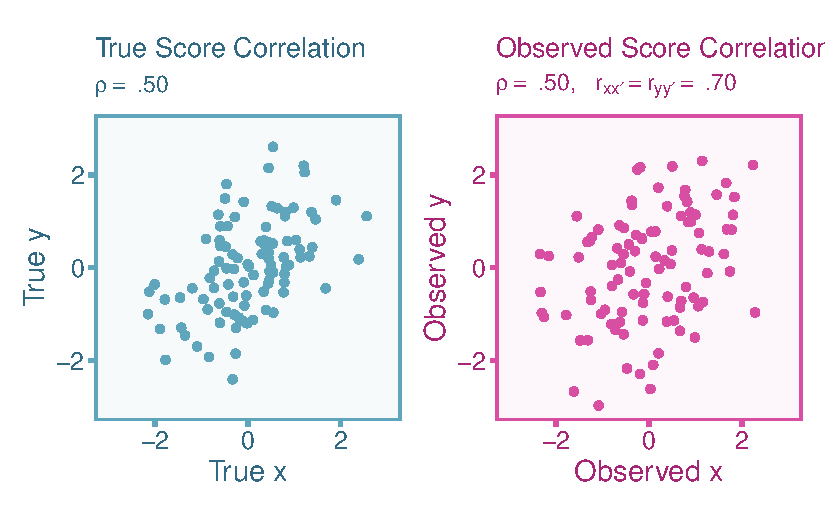
\includegraphics{unreliability_files/figure-pdf/unnamed-chunk-15-1.pdf}

}

\end{figure}

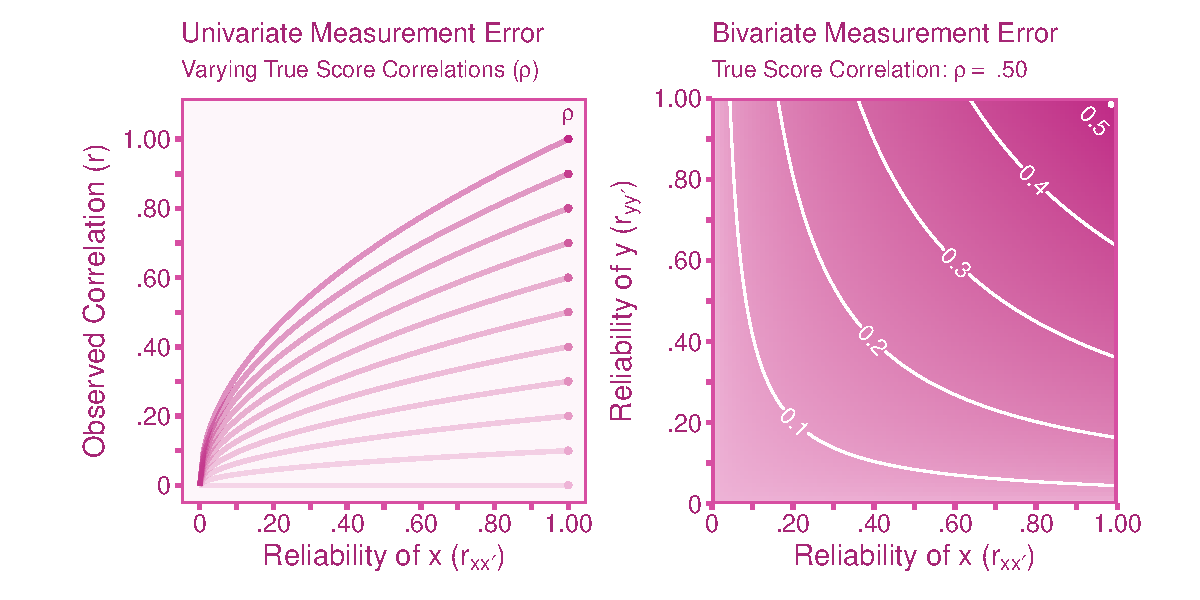
\includegraphics{unreliability_files/figure-pdf/unnamed-chunk-16-1.pdf}

Ultimately, the inflation of the observed standard deviation As
described in Equation~\ref{eq-reliability}, the reliability can be
interpreted as the ratio of total observed variance to

Fortunately, there are corrections that can be applied to effect size
estimates to account for bias.

\hypertarget{corrections-for-bias-in-correlations}{%
\section{Corrections for Bias in
Correlations}\label{corrections-for-bias-in-correlations}}

\hypertarget{correction-for-unreliability-in-correlation-coefficients}{%
\section{Correction for Unreliability in Correlation
Coefficients}\label{correction-for-unreliability-in-correlation-coefficients}}

\hypertarget{bias-in-correlations}{%
\subsection{Bias in Correlations}\label{bias-in-correlations}}

Measurements that produce scores with low reliability by definition have
low correlations between observed scores on parallel forms of the
measurement. It should should not be expected that any other variable
would.

\hypertarget{bias-in-standardized-mean-difference}{%
\subsection{Bias in Standardized Mean
Difference}\label{bias-in-standardized-mean-difference}}

\hypertarget{between-group-standardized-mean-difference}{%
\subsubsection{Between-Group Standardized Mean
Difference}\label{between-group-standardized-mean-difference}}

\hypertarget{repeated-measures-standardized-mean-difference}{%
\subsubsection{Repeated Measures Standardized Mean
Difference}\label{repeated-measures-standardized-mean-difference}}

(Haertel 2006)

(F. L. Schmidt, Le, and Ilies 2003)

(Gliem and Gliem 2003)

(Bobko, Roth, and Bobko 2001)

(Mendoza and Mumford 1987)

(Brennan 2010)

(Viswanathan 2005)

(Viswesvaran et al. 2014)

(Sijtsma 2009)

(Charles 2005)

(Spearman 1904)

\hypertarget{misclassification}{%
\chapter{Misclassification}\label{misclassification}}

(Chyou 2007)

(Wiernik and Dahlke 2020)

(John E. Hunter and Schmidt 1990)

\hypertarget{artificial-dichotomization}{%
\chapter{Artificial Dichotomization}\label{artificial-dichotomization}}

(Naggara et al. 2011)

(Russell, Pinto, and Bobko 1991)

(Digby 1983)

(Maxwell and Delaney 1993)

(J. Hunter and Schmidt 1990)

(Vargha et al. 1996)

(Royston, Altman, and Sauerbrei 2006)

(Peters and Voorhis 1940)

(Bonett and Price 2005)

(Ulrich and Wirtz 2004)

(Muthén and Hofacker 1988)

(MacCallum et al. 2002)

\hypertarget{scale-coarseness}{%
\chapter{Scale Coarseness}\label{scale-coarseness}}

(Symonds 1924)

(Aguinis, Pierce, and Culpepper 2009)

(Krieg 1999)

\hypertarget{direct-range-restrictionenhancement}{%
\chapter{Direct Range
Restriction/Enhancement}\label{direct-range-restrictionenhancement}}

(Bobko, Roth, and Bobko 2001)

(Sackett and Yang 2000)

(Law, Schmidt, and Hunter 1994)

(Thorndike 1949)

(John E. Hunter and Schmidt 1990)

(Wiernik and Dahlke 2020)

\hypertarget{indirect-range-restrictionenhancement}{%
\chapter{Indirect Range
Restriction/Enhancement}\label{indirect-range-restrictionenhancement}}

(Dahlke and Wiernik 2020)

(John E. Hunter and Schmidt 1990)

(Thorndike 1949)

(Bobko, Roth, and Bobko 2001)

(Sackett and Yang 2000)

\part{Application to Meta-Analysis}

\hypertarget{introduction-to-meta-analysis-methods}{%
\chapter{Introduction to Meta-Analysis
Methods}\label{introduction-to-meta-analysis-methods}}

\hypertarget{fixed-effects-model}{%
\section{Fixed Effects Model}\label{fixed-effects-model}}

\hypertarget{random-effects-model}{%
\section{Random Effects Model}\label{random-effects-model}}

(Borenstein et al. 2010)

(Hartung 1999)

(Cooper, Hedges, and Valentine 2009)

(DerSimonian and Kacker 2007)

\hypertarget{artifact-correction-meta-analysis}{%
\chapter{Artifact Correction
Meta-Analysis}\label{artifact-correction-meta-analysis}}

\hypertarget{individual-artifact-correction-model}{%
\section{Individual Artifact Correction
Model}\label{individual-artifact-correction-model}}

\hypertarget{artifact-distribution-model}{%
\section{Artifact Distribution
Model}\label{artifact-distribution-model}}

\hypertarget{alternative-methods}{%
\section{Alternative Methods}\label{alternative-methods}}

(John E. Hunter and Schmidt 1990)

(Wiernik and Dahlke 2020)

(F. Schmidt and Hunter 1977)

(Murphy 2003)

(Viswesvaran and Ones 1995)

(Raju and Burke 1983)

(Callender and Osburn 1980)

\bookmarksetup{startatroot}

\hypertarget{references}{%
\chapter*{References}\label{references}}
\addcontentsline{toc}{chapter}{References}

\markboth{References}{References}

\hypertarget{refs}{}
\begin{CSLReferences}{1}{0}
\leavevmode\vadjust pre{\hypertarget{ref-aguinis2009}{}}%
Aguinis, Herman, Charles A Pierce, and Steven A Culpepper. 2009.
{``Scale Coarseness as a Methodological Artifact,''} September.

\leavevmode\vadjust pre{\hypertarget{ref-bobko2001}{}}%
Bobko, Philip, Philip Roth, and Christopher Bobko. 2001. {``Correcting
the Effect Size of d for Range Restriction and Unreliability.''}
\emph{Organizational Research Methods - ORGAN RES METHODS} 4 (January):
46--61. \url{https://doi.org/10.1177/109442810141003}.

\leavevmode\vadjust pre{\hypertarget{ref-bonett2005}{}}%
Bonett, Douglas G., and Robert M. Price. 2005. {``Inferential Methods
for the Tetrachoric Correlation Coefficient.''} \emph{Journal of
Educational and Behavioral Statistics} 30 (2): 213--25.
\url{https://www.jstor.org/stable/3701350}.

\leavevmode\vadjust pre{\hypertarget{ref-borenstein2010}{}}%
Borenstein, Michael, Larry V. Hedges, Julian P. T. Higgins, and Hannah
R. Rothstein. 2010. {``A Basic Introduction to Fixed-Effect and
Random-Effects Models for Meta-Analysis.''} \emph{Research Synthesis
Methods} 1 (2): 97--111. \url{https://doi.org/10.1002/jrsm.12}.

\leavevmode\vadjust pre{\hypertarget{ref-brennan2010}{}}%
Brennan, Robert L. 2010. {``Generalizability Theory and Classical Test
Theory.''} \emph{Applied Measurement in Education} 24 (1): 1--21.
\url{https://doi.org/10.1080/08957347.2011.532417}.

\leavevmode\vadjust pre{\hypertarget{ref-callender1980}{}}%
Callender, John C., and H. G. Osburn. 1980. {``Development and Test of a
New Model for Validity Generalization.''} \emph{Journal of Applied
Psychology} 65 (5): 543--58.
\url{https://doi.org/10.1037/0021-9010.65.5.543}.

\leavevmode\vadjust pre{\hypertarget{ref-charles2005}{}}%
Charles, Eric. 2005. {``The Correction for Attenuation Due to
Measurement Error: Clarifying Concepts and Creating Confidence Sets.''}
\emph{Psychological Methods} 10 (July): 206--26.
\url{https://doi.org/10.1037/1082-989X.10.2.206}.

\leavevmode\vadjust pre{\hypertarget{ref-chyou2007}{}}%
Chyou, Po-Huang. 2007. {``Patterns of Bias Due to Differential
Misclassification by Case{\textendash}control Status in a
Case{\textendash}control Study.''} \emph{European Journal of
Epidemiology} 22 (1): 7--17.
\url{https://doi.org/10.1007/s10654-006-9078-x}.

\leavevmode\vadjust pre{\hypertarget{ref-thehand2009}{}}%
Cooper, Harris M., Larry V. Hedges, and Jeff C. Valentine, eds. 2009.
\emph{The Handbook of Research Synthesis and Meta-Analysis}. 2nd ed. New
York: Russell Sage Foundation.

\leavevmode\vadjust pre{\hypertarget{ref-dahlke2019}{}}%
Dahlke, Jeffrey A., and Brenton M. Wiernik. 2019. {``Psychmeta: An R
Package for Psychometric Meta-Analysis.''} \emph{Applied Psychological
Measurement} 43 (5): 415--16.
\url{https://doi.org/10.1177/0146621618795933}.

\leavevmode\vadjust pre{\hypertarget{ref-dahlke2020}{}}%
---------. 2020. {``Not Restricted to Selection Research: Accounting for
Indirect Range Restriction in Organizational Research.''}
\emph{Organizational Research Methods} 23 (4): 717--49.
\url{https://doi.org/10.1177/1094428119859398}.

\leavevmode\vadjust pre{\hypertarget{ref-dersimonian2007}{}}%
DerSimonian, Rebecca, and Raghu N. Kacker. 2007. {``Random-Effects Model
for Meta-Analysis of Clinical Trials: An Update.''} \emph{NIST} 28
(January): 105--14.
\url{https://www.nist.gov/publications/random-effects-model-meta-analysis-clinical-trials-update}.

\leavevmode\vadjust pre{\hypertarget{ref-digby1983}{}}%
Digby, P. G. N. 1983. {``Approximating the Tetrachoric Correlation
Coefficient.''} \emph{Biometrics} 39 (3): 753--57.
\url{https://doi.org/10.2307/2531104}.

\leavevmode\vadjust pre{\hypertarget{ref-fisher1915}{}}%
Fisher, R. A. 1915. {``Frequency Distribution of the Values of the
Correlation Coefficient in Samples from an Indefinitely Large
Population.''} \emph{Biometrika} 10 (4): 507--21.
\url{https://doi.org/10.2307/2331838}.

\leavevmode\vadjust pre{\hypertarget{ref-galton1907}{}}%
Galton, Francis. 1907. {``Vox Populi.''} \emph{Nature} 75 (1949):
450--51. \url{https://doi.org/10.1038/075450a0}.

\leavevmode\vadjust pre{\hypertarget{ref-gliem2003}{}}%
Gliem, Joseph A., and Rosemary R. Gliem. 2003. {``Calculating,
Interpreting, And Reporting Cronbach{'}s Alpha Reliability Coefficient
For Likert-Type Scales.''}
\url{https://scholarworks.iupui.edu/handle/1805/344}.

\leavevmode\vadjust pre{\hypertarget{ref-haertel2006}{}}%
Haertel, Edward H. 2006. {``3. Reliability.''} In, 4th ed.

\leavevmode\vadjust pre{\hypertarget{ref-hartung1999}{}}%
Hartung, Joachim. 1999. {``An Alternative Method for Meta-Analysis.''}
\emph{Biometrical Journal} 41 (8): 901--16.
\url{https://doi.org/10.1002/(SICI)1521-4036(199912)41:8\%3C901::AID-BIMJ901\%3E3.0.CO;2-W}.

\leavevmode\vadjust pre{\hypertarget{ref-hedges1981}{}}%
Hedges, Larry V. 1981. {``Distribution Theory for Glass's Estimator of
Effect Size and Related Estimators.''} \emph{Journal of Educational
Statistics} 6 (2): 107--28.
\url{https://doi.org/10.3102/10769986006002107}.

\leavevmode\vadjust pre{\hypertarget{ref-hedges1989}{}}%
---------. 1989. {``An Unbiased Correction for Sampling Error in
Validity Generalization Studies.''} \emph{Journal of Applied Psychology}
74 (3): 469--77. \url{https://doi.org/10.1037/0021-9010.74.3.469}.

\leavevmode\vadjust pre{\hypertarget{ref-hunter}{}}%
Hunter, John E, and Ronda F Hunter. n.d. {``Validity and Utility of
Alternative Predictors of Job Performance.''}

\leavevmode\vadjust pre{\hypertarget{ref-hunter1990a}{}}%
Hunter, John E., and Frank L. Schmidt. 1990. \emph{Methods of
meta-analysis: correcting error and bias in research findings}. Newbury
Park: Sage Publications.

\leavevmode\vadjust pre{\hypertarget{ref-hunter1990}{}}%
Hunter, John, and Frank Schmidt. 1990. {``Dichotomization of Continuous
Variables: The Implications for Meta-Analysis.''} \emph{Journal of
Applied Psychology} 75 (June): 334--49.
\url{https://doi.org/10.1037/0021-9010.75.3.334}.

\leavevmode\vadjust pre{\hypertarget{ref-krieg1999}{}}%
Krieg, Edward F. 1999. {``Biases Induced by Coarse Measurement
Scales.''} \emph{Educational and Psychological Measurement} 59 (5):
749--66. \url{https://doi.org/10.1177/00131649921970125}.

\leavevmode\vadjust pre{\hypertarget{ref-law1994}{}}%
Law, Kenneth, Frank Schmidt, and John Hunter. 1994. {``Nonlinearity of
Range Corrections in Meta-Analysis: Test of an Improved Procedure.''}
\emph{Journal of Applied Psychology} 79 (December): 978--86.
\url{https://doi.org/10.1037/0021-9010.79.6.978}.

\leavevmode\vadjust pre{\hypertarget{ref-lin2018}{}}%
Lin, Lifeng. 2018. {``Bias Caused by Sampling Error in Meta-Analysis
with Small Sample Sizes.''} \emph{PLOS ONE} 13 (9): e0204056.
\url{https://doi.org/10.1371/journal.pone.0204056}.

\leavevmode\vadjust pre{\hypertarget{ref-maccallum2002}{}}%
MacCallum, Robert C., Shaobo Zhang, Kristopher J. Preacher, and Derek D.
Rucker. 2002. {``On the Practice of Dichotomization of Quantitative
Variables.''} \emph{Psychological Methods} 7: 19--40.
\url{https://doi.org/10.1037/1082-989X.7.1.19}.

\leavevmode\vadjust pre{\hypertarget{ref-maxwell1993}{}}%
Maxwell, Scott, and Harold Delaney. 1993. {``Bivariate Median Splits and
Spurious Statistical Significance.''} \emph{Psychological Bulletin} 113
(January): 181--90. \url{https://doi.org/10.1037/0033-2909.113.1.181}.

\leavevmode\vadjust pre{\hypertarget{ref-mendoza1987}{}}%
Mendoza, Jorge L., and Michael Mumford. 1987. {``Corrections for
Attenuation and Range Restriction on the Predictor.''} \emph{Journal of
Educational Statistics} 12 (3): 282--93.
\url{https://doi.org/10.3102/10769986012003282}.

\leavevmode\vadjust pre{\hypertarget{ref-murphy2003}{}}%
Murphy, Kevin R. 2003. \emph{Validity Generalization: A Critical
Review}. Psychology Press.

\leavevmode\vadjust pre{\hypertarget{ref-muthuxe9n1988}{}}%
Muthén, Bengt, and Charles Hofacker. 1988. {``Testing the Assumptions
Underlying Tetrachoric Correlations.''} \emph{Psychometrika} 53 (4):
563--77. \url{https://doi.org/10.1007/BF02294408}.

\leavevmode\vadjust pre{\hypertarget{ref-naggara2011}{}}%
Naggara, O., J. Raymond, F. Guilbert, D. Roy, A. Weill, and D. G.
Altman. 2011. {``Analysis by Categorizing or Dichotomizing Continuous
Variables Is Inadvisable: An Example from the Natural History of
Unruptured Aneurysms.''} \emph{American Journal of Neuroradiology} 32
(3): 437--40. \url{https://doi.org/10.3174/ajnr.A2425}.

\leavevmode\vadjust pre{\hypertarget{ref-olkin1958}{}}%
Olkin, Ingram, and John W. Pratt. 1958. {``Unbiased Estimation of
Certain Correlation Coefficients.''} \emph{The Annals of Mathematical
Statistics} 29 (1): 201--11. \url{https://www.jstor.org/stable/2237306}.

\leavevmode\vadjust pre{\hypertarget{ref-peters1940}{}}%
Peters, Charles C., and Walter R. Van Voorhis. 1940. {``Further Methods
of Correlation.''} In, 362--403. New York, NY, US: McGraw-Hill Book
Company. \url{https://doi.org/10.1037/13596-013}.

\leavevmode\vadjust pre{\hypertarget{ref-raju1983}{}}%
Raju, Nambury, and Michael Burke. 1983. {``Two Procedures for Studying
Validity Generalization.''} \emph{Journal of Applied Psychology} 68
(August): 382--95. \url{https://doi.org/10.1037/0021-9010.68.3.382}.

\leavevmode\vadjust pre{\hypertarget{ref-roth2015}{}}%
Roth, Bettina. 2015. {``Intelligence and School Grades: A
Meta-Analysis.''}

\leavevmode\vadjust pre{\hypertarget{ref-royston2006}{}}%
Royston, Patrick, Douglas G. Altman, and Willi Sauerbrei. 2006.
{``Dichotomizing Continuous Predictors in Multiple Regression: A Bad
Idea.''} \emph{Statistics in Medicine} 25 (1): 127--41.
\url{https://doi.org/10.1002/sim.2331}.

\leavevmode\vadjust pre{\hypertarget{ref-russell1991}{}}%
Russell, Craig J., Jeffrey K. Pinto, and Philip Bobko. 1991.
{``Appropriate Moderated Regression and Inappropriate Research Strategy:
A Demonstration of Information Loss Due to Scale Coarseness''} 15 (3):
257--66. \url{https://doi.org/10.1177/014662169101500305}.

\leavevmode\vadjust pre{\hypertarget{ref-sackett2000}{}}%
Sackett, Paul R., and Hyuckseung Yang. 2000. {``Correction for Range
Restriction: An Expanded Typology.''} \emph{Journal of Applied
Psychology} 85 (1): 112--18.
\url{https://doi.org/10.1037/0021-9010.85.1.112}.

\leavevmode\vadjust pre{\hypertarget{ref-schmidt2003}{}}%
Schmidt, Frank L., Huy Le, and Remus Ilies. 2003. {``Beyond Alpha: An
Empirical Examination of the Effects of Different Sources of Measurement
Error on Reliability Estimates for Measures of Individual-Differences
Constructs.''} \emph{Psychological Methods} 8: 206--24.
\url{https://doi.org/10.1037/1082-989X.8.2.206}.

\leavevmode\vadjust pre{\hypertarget{ref-schmidt1977}{}}%
Schmidt, Frank, and John Hunter. 1977. {``Development of a General
Solution to the Problem of Validity Generalization.''} \emph{Journal of
Applied Psychology} 62 (October): 529--40.
\url{https://doi.org/10.1037/0021-9010.62.5.529}.

\leavevmode\vadjust pre{\hypertarget{ref-sijtsma2009}{}}%
Sijtsma, Klaas. 2009. {``On the Use, the Misuse, and the Very Limited
Usefulness of~Cronbach{'}s Alpha.''} \emph{Psychometrika} 74 (1):
107--20. \url{https://doi.org/10.1007/s11336-008-9101-0}.

\leavevmode\vadjust pre{\hypertarget{ref-spearman1904}{}}%
Spearman, C. 1904. {``The Proof and Measurement of Association Between
Two Things.''} \emph{International Journal of Epidemiology} 39 (5):
1137--50. \url{https://doi.org/10.1093/ije/dyq191}.

\leavevmode\vadjust pre{\hypertarget{ref-symonds1924}{}}%
Symonds, P. M. 1924. {``On the Loss of Reliability in Ratings Due to
Coarseness of the Scale.''} \emph{Journal of Experimental Psychology} 7
(6): 456--61. \url{https://doi.org/10.1037/h0074469}.

\leavevmode\vadjust pre{\hypertarget{ref-thorndike1949}{}}%
Thorndike, Robert L. 1949. \emph{Personnel Selection; Test and
Measurement Techniques}. Personnel Selection; Test and Measurement
Techniques. Oxford, England: Wiley.

\leavevmode\vadjust pre{\hypertarget{ref-ulrich2004}{}}%
Ulrich, Rolf, and Markus Wirtz. 2004. {``On the Correlation of a
Naturally and an Artificially Dichotomized Variable.''} \emph{British
Journal of Mathematical and Statistical Psychology} 57 (2): 235--51.
\url{https://doi.org/10.1348/0007110042307203}.

\leavevmode\vadjust pre{\hypertarget{ref-vanaarde2017}{}}%
Van Aarde, Ninette, Deon Meiring, and Brenton M. Wiernik. 2017. {``The
Validity of the Big Five Personality Traits for Job Performance:
Meta{-}Analyses of South African Studies.''} \emph{International Journal
of Selection and Assessment} 25 (3): 223--39.
\url{https://doi.org/10.1111/ijsa.12175}.

\leavevmode\vadjust pre{\hypertarget{ref-vargha1996}{}}%
Vargha, András, Tamás Rudas, Harold D. Delaney, and Scott E. Maxwell.
1996. {``Dichotomization, Partial Correlation, and Conditional
Independence.''} \emph{Journal of Educational and Behavioral Statistics}
21 (3): 264--82. \url{https://doi.org/10.2307/1165272}.

\leavevmode\vadjust pre{\hypertarget{ref-viswanathan2005}{}}%
Viswanathan, Madhu. 2005. \emph{Measurement Error and Research Design}.
SAGE.

\leavevmode\vadjust pre{\hypertarget{ref-viswesvaran1995}{}}%
Viswesvaran, Chockalingam, and Deniz S. Ones. 1995. {``Theory Testing:
Combining Psychometric Meta-Analysis and Structural Equations
Modeling.''} \emph{Personnel Psychology} 48 (4): 865--85.
\url{https://doi.org/10.1111/j.1744-6570.1995.tb01784.x}.

\leavevmode\vadjust pre{\hypertarget{ref-viswesvaran2014}{}}%
Viswesvaran, Chockalingam, Deniz S. Ones, Frank L. Schmidt, Huy Le, and
In-Sue Oh. 2014. {``Measurement Error Obfuscates Scientific Knowledge:
Path to Cumulative Knowledge Requires Corrections for Unreliability and
Psychometric Meta-Analyses.''} \emph{Industrial and Organizational
Psychology} 7 (4): 507--18.
\url{https://doi.org/10.1017/S1754942600006799}.

\leavevmode\vadjust pre{\hypertarget{ref-wiernik2020}{}}%
Wiernik, Brenton M., and Jeffrey A. Dahlke. 2020. {``Obtaining Unbiased
Results in Meta-Analysis: The Importance of Correcting for Statistical
Artifacts.''} \emph{Advances in Methods and Practices in Psychological
Science} 3 (1): 94--123. \url{https://doi.org/10.1177/2515245919885611}.

\end{CSLReferences}



\end{document}
